        %%******************************************%%
        %%                                          %%
        %%        Modello di tesi di laurea         %%
        %%            di Andrea Giraldin            %%
        %%                                          %%
        %%             2 novembre 2012              %%
        %%                                          %%
        %%******************************************%%


% I seguenti commenti speciali impostano:
% 1. 
% 2. PDFLaTeX come motore di composizione;
% 3. tesi.tex come documento principale;
% 4. il controllo ortografico italiano per l'editor.

% !TEX encoding = UTF-8
% !TEX TS-program = pdflatex
% !TEX root = tesi.tex
% !TEX spellcheck = it-IT

\documentclass[10pt,                    % corpo del font principale
               a4paper,                 % carta A4
               twoside,                 % impagina per fronte-retro
               openright,               % inizio capitoli a destra
               english,                 
               italian,                 
               ]{book}    

\usepackage[utf8]{inputenc}             % codifica di input; anche [latin1] va bene
                                        % NOTA BENE! va accordata con le preferenze dell'editor

%**************************************************************
% Importazione package
%************************************************************** 

%\usepackage{amsmath,amssymb,amsthm}    % matematica

\usepackage[english, italian]{babel}    % per scrivere in italiano e in inglese;
                                        % l'ultima lingua (l'italiano) risulta predefinita

\usepackage{bookmark}                   % segnalibri

\usepackage{caption}                    % didascalie

\usepackage{chngpage,calc}              % centra il frontespizio

\usepackage{csquotes}                   % gestisce automaticamente i caratteri (")

\usepackage{emptypage}                  % pagine vuote senza testatina e piede di pagina

\usepackage{epigraph}					% per epigrafi

\usepackage{eurosym}                    % simbolo dell'euro

\usepackage[T1]{fontenc}                % codifica dei font:
                                        % NOTA BENE! richiede una distribuzione *completa* di LaTeX

%\usepackage{indentfirst}               % rientra il primo paragrafo di ogni sezione

\usepackage{graphicx}                   % immagini

\usepackage{hyperref}                   % collegamenti ipertestuali



\usepackage[binding=5mm]{layaureo}      % margini ottimizzati per l'A4; rilegatura di 5 mm

\usepackage{listings}                   % codici

\usepackage{microtype}                  % microtipografia

\usepackage{mparhack,fixltx2e,relsize}  % finezze tipografiche

\usepackage{nameref}                    % visualizza nome dei riferimenti                                      

\usepackage[font=small]{quoting}        % citazioni

\usepackage{subfig}                     % sottofigure, sottotabelle

\usepackage[italian]{varioref}          % riferimenti completi della pagina

\usepackage[dvipsnames]{xcolor}         % colori

\usepackage{booktabs}                   % tabelle                                       
\usepackage{tabularx}                   % tabelle di larghezza prefissata                                    
\usepackage{longtable}                  % tabelle su più pagine                                        
\usepackage{ltxtable}                   % tabelle su più pagine e adattabili in larghezza

\usepackage[toc, acronym]{glossaries}   % glossario
                                        % per includerlo nel documento bisogna:
                                        % 1. compilare una prima volta tesi.tex;
                                        % 2. eseguire: makeindex -s tesi.ist -t tesi.glg -o tesi.gls tesi.glo
                                        % 3. eseguire: makeindex -s tesi.ist -t tesi.alg -o tesi.acr tesi.acn
                                        % 4. compilare due volte tesi.tex.

\usepackage[backend=biber,style=verbose-ibid,hyperref,backref]{biblatex}
                                        % eccellente pacchetto per la bibliografia; 
                                        % produce uno stile di citazione autore-anno; 
                                        % lo stile "numeric-comp" produce riferimenti numerici
                                        % per includerlo nel documento bisogna:
                                        % 1. compilare una prima volta tesi.tex;
                                        % 2. eseguire: biber tesi
                                        % 3. compilare ancora tesi.tex.

%**************************************************************
% file contenente le impostazioni della tesi
%**************************************************************

%**************************************************************
% Frontespizio
%**************************************************************

% Autore
\newcommand{\myName}{Tomas Mali}                                    
\newcommand{\myTitle}{Progettazione e implementazione di una soluzione BI per la gestione di processi di budget }

% Tipo di tesi                   
\newcommand{\myDegree}{Tesi di laurea triennale}

% Università             
\newcommand{\myUni}{Università degli Studi di Padova}

% Facoltà       
\newcommand{\myFaculty}{Corso di Laurea in Informatica}

% Dipartimento
\newcommand{\myDepartment}{Dipartimento di Matematica "Tullio Levi-Civita"}

% Titolo del relatore
\newcommand{\profTitle}{Prof.}

% Relatore
\newcommand{\myProf}{Bujari Armir}

% Luogo
\newcommand{\myLocation}{Padova}

% Anno accademico
\newcommand{\myAA}{2017-2018}

% Data discussione
\newcommand{\myTime}{Aprile 2018}


%**************************************************************
% Impostazioni di impaginazione
% see: http://wwwcdf.pd.infn.it/AppuntiLinux/a2547.htm
%**************************************************************

\setlength{\parindent}{14pt}   % larghezza rientro della prima riga
\setlength{\parskip}{0pt}   % distanza tra i paragrafi


%**************************************************************
% Impostazioni di biblatex
%**************************************************************
\bibliography{bibliografia} % database di biblatex 

\defbibheading{bibliography} {
    \cleardoublepage
    \phantomsection 
    \addcontentsline{toc}{chapter}{\bibname}
    \chapter*{\bibname\markboth{\bibname}{\bibname}}
}

\setlength\bibitemsep{1.5\itemsep} % spazio tra entry

\DeclareBibliographyCategory{opere}
\DeclareBibliographyCategory{web}

\addtocategory{opere}{womak:lean-thinking}
\addtocategory{web}{site:agile-manifesto}

\defbibheading{opere}{\section*{Riferimenti bibliografici}}
\defbibheading{web}{\section*{Siti Web consultati}}


%**************************************************************
% Impostazioni di caption
%**************************************************************
\captionsetup{
    tableposition=top,
    figureposition=bottom,
    font=small,
    format=hang,
    labelfont=bf
}

%**************************************************************
% Impostazioni di glossaries
%**************************************************************

%**************************************************************
% Acronimi
%**************************************************************
\renewcommand{\acronymname}{Acronimi e abbreviazioni}

\newacronym[description={\glslink{apig}{Application Program Interface}}]
    {api}{API}{Application Program Interface}

\newacronym[description={\glslink{umlg}{Unified Modeling Language}}]
    {uml}{UML}{Unified Modeling Language}

%**************************************************************
% Glossario
%**************************************************************
%\renewcommand{\glossaryname}{Glossario}





\newglossaryentry{B2B}
{
    name=\glslink{B2B}{B2B},
    text=B2B,
    description={Acronimo di Business-to-Business, in italiano commercio interaziendale, sta ad indicare le transizioni elettroniche tra imprese.}
}

\newglossaryentry{Business Intelligence}
{
    name=\glslink{Business Intelligence}{BUSINESS INTELLIGENCE},
    text= Business Intelligence,
    description={Con questa locuzione si fa riferimento ad un insieme di processi aziendali per raccogleire dati ed analizzare informazioni strategiche, tecnologie utilizzate per realizzare questi processi e le informazioni ottenute come risultato di questi processi.}
}

\newglossaryentry{DAO}
{
    name=\glslink{DAO}{DAO},
    text= DAO,
    description={Acronimo di Data Acess Object, è un pattern architetturale per la gestione della persistenza: si tratta fondamentalmente di una classe con relativi metodi che rappresenta un'entitaà tabellare di un database relazionale, usat principalmente in applicazioni web. Il vantaggio relativo all'uso del DAO è dunque il mantenimento di una rigida separazione tra le componenti di un'applicazione.}
}
\newglossaryentry{data-layer}
{
    name=\glslink{data-layer}{Data-Layer},
    text= data-layer,
    description={E' uno strato di una applicazione che fornisce un accesso semplificato ai dati memorizzati nell'archiviazione persistente, come un database relazionale.}
}
\newglossaryentry{framework}
{
    name=\glslink{framework}{FRAMEWORK},
    text= framework,
    description={ Un framework, termine della lingua inglese che può essere tradotto come struttura, in informatica e specificatamente nello sviluppo software, è un'architettura logica di supporto (spesso un'implementazione logica di un particolare design pattern) su cui un software può essere progettato e realizzato, spesso facilitandone lo sviluppo da parte del programmatore.}
}
\newglossaryentry{IDE}
{
    name=\glslink{IDE}{IDE},
    text= IDE,
    description={In informatica un ambiente di sviluppo integrato è un software che, in fase di programmazione, aiuta i programmatori nello sviluppo del codice sorgente di un programma. Spesso l'IDE aiuta lo sviluppatore segnalando errori di sintassi del codice direttamente in fase di scrittura, oltre a tutta una serie di strumenti e funzionalità di supporto alla fase di sviluppo e debugging.}
}

\newglossaryentry{Open Power Foundation IBM}
{
    name=\glslink{Open Power Foundation IBM}{OPEN POWER FOUNDATION IBM},
    text= Open Power Foundation IBM,
    description={Open-Power Foundation è una collaborazione intorno ai prodotti di Power Architecture avviati da IBM e annunciata come Open-Power Consortium il 6 agosto 2013. IBM sta aprendo la tecnologia che circonda le offerte di Power Architecture come specifiche del processore, firmware e software e offre questo su una licenza free utilizzando un modello di sviluppo collaborativo con i loro partner.}
}




\newglossaryentry{open source}
{
    name=\glslink{open source}{OPEN SOURCE},
    text= open source,
    description={In informatica, il termine inglese open source (che significa sorgente aperta) indica un software di cui gli autori (più precisamente, i detentori dei diritti) rendono pubblico il codice sorgente, favorendone il libero studio e permettendo a programmatori indipendenti di apportarvi modifiche ed estensioni.}
}

\newglossaryentry{plug-in}
{
    name=\glslink{plug-in}{PLUG-IN},
    text= plug-in,
    description={Il plugin in campo informatico è un programma non autonomo che interagisce con un altro programma per ampliarne o estenderne le funzionalità originarie. Ad esempio, un plugin per un software di grafica permette l'utilizzo di nuove funzioni non presenti nel software principale}
}


\newglossaryentry{UML2.0}
{
    name=\glslink{UML2.0}{UML2.0},
    text= UML2.0,
    description={In ingegneria del software, UML (unified modeling language, "linguaggio di modellizzazione unificato") è un linguaggio di modellizzazione e specifica basato
sul paradigma orientato agli oggetti. La versione 2.0 è stata consolidata nel 2004 e ufficializzata nel 2005. UML 2.0 riorganizza molti degli elementi della versione precedente in un quadro di riferimento ampliato e introduce molti nuovi strumenti, inclusi alcuni nuovi tipi di diagrammi }
}



\newglossaryentry{Use Cases Diagram}
{
    name=\glslink{Use Cases Diagram}{USE CASES DIAGRAM},
    text= Use Cases Diagram,
    description={ In UML, gli Use Case Diagram (UCD o diagrammi dei casi d'uso) sono diagrammi dedicati alla descrizione delle funzioni o servizi offerti da un sistema, cosi come sono percepiti e utilizzati dagli attori che interagiscono col sistema stesso.}
}










 % database di termini
\makeglossaries


%**************************************************************
% Impostazioni di graphicx
%**************************************************************
\graphicspath{{immagini/}} % cartella dove sono riposte le immagini


%**************************************************************
% Impostazioni di hyperref
%**************************************************************
\hypersetup{
    %hyperfootnotes=false,
    %pdfpagelabels,
    %draft,	% = elimina tutti i link (utile per stampe in bianco e nero)
    colorlinks=true,
    linktocpage=true,
    pdfstartpage=1,
    pdfstartview=FitV,
    % decommenta la riga seguente per avere link in nero (per esempio per la stampa in bianco e nero)
    %colorlinks=false, linktocpage=false, pdfborder={0 0 0}, pdfstartpage=1, pdfstartview=FitV,
    breaklinks=true,
    pdfpagemode=UseNone,
    pageanchor=true,
    pdfpagemode=UseOutlines,
    plainpages=false,
    bookmarksnumbered,
    bookmarksopen=true,
    bookmarksopenlevel=1,
    hypertexnames=true,
    pdfhighlight=/O,
    %nesting=true,
    %frenchlinks,
    urlcolor=webbrown,
    linkcolor=RoyalBlue,
    citecolor=webgreen,
    %pagecolor=RoyalBlue,
    %urlcolor=Black, linkcolor=Black, citecolor=Black, %pagecolor=Black,
    pdftitle={\myTitle},
    pdfauthor={\textcopyright\ \myName, \myUni, \myFaculty},
    pdfsubject={},
    pdfkeywords={},
    pdfcreator={pdfLaTeX},
    pdfproducer={LaTeX}
}

%**************************************************************
% Impostazioni di itemize
%**************************************************************
\renewcommand{\labelitemi}{$\ast$}

%\renewcommand{\labelitemi}{$\bullet$}
%\renewcommand{\labelitemii}{$\cdot$}
%\renewcommand{\labelitemiii}{$\diamond$}
%\renewcommand{\labelitemiv}{$\ast$}


%**************************************************************
% Impostazioni di listings
%**************************************************************
\lstset{
    language=[LaTeX]Tex,%C++,
    keywordstyle=\color{RoyalBlue}, %\bfseries,
    basicstyle=\small\ttfamily,
    %identifierstyle=\color{NavyBlue},
    commentstyle=\color{Green}\ttfamily,
    stringstyle=\rmfamily,
    numbers=none, %left,%
    numberstyle=\scriptsize, %\tiny
    stepnumber=5,
    numbersep=8pt,
    showstringspaces=false,
    breaklines=true,
    frameround=ftff,
    frame=single
} 


%**************************************************************
% Impostazioni di xcolor
%**************************************************************
\definecolor{webgreen}{rgb}{0,.5,0}
\definecolor{webbrown}{rgb}{.6,0,0}


%**************************************************************
% Altro
%**************************************************************

\newcommand{\omissis}{[\dots\negthinspace]} % produce [...]

% eccezioni all'algoritmo di sillabazione
\hyphenation
{
    ma-cro-istru-zio-ne
    gi-ral-din
}

\newcommand{\sectionname}{sezione}
\addto\captionsitalian{\renewcommand{\figurename}{Figura}
                       \renewcommand{\tablename}{Tabella}}

\newcommand{\glsfirstoccur}{\ap{{[g]}}}

\newcommand{\intro}[1]{\emph{\textsf{#1}}}

%**************************************************************
% Environment per ``rischi''
%**************************************************************
\newcounter{riskcounter}                % define a counter
\setcounter{riskcounter}{0}             % set the counter to some initial value

%%%% Parameters
% #1: Title
\newenvironment{risk}[1]{
    \refstepcounter{riskcounter}        % increment counter
    \par \noindent                      % start new paragraph
    \textbf{\arabic{riskcounter}. #1}   % display the title before the 
                                        % content of the environment is displayed 
}{
    \par\medskip
}

\newcommand{\riskname}{Rischio}

\newcommand{\riskdescription}[1]{\textbf{\\Descrizione:} #1.}

\newcommand{\risksolution}[1]{\textbf{\\Soluzione:} #1.}

%**************************************************************
% Environment per ``use case''
%**************************************************************
\newcounter{usecasecounter}             % define a counter
\setcounter{usecasecounter}{0}          % set the counter to some initial value

%%%% Parameters
% #1: ID
% #2: Nome
\newenvironment{usecase}[2]{
    \renewcommand{\theusecasecounter}{\usecasename #1}  % this is where the display of 
                                                        % the counter is overwritten/modified
    \refstepcounter{usecasecounter}             % increment counter
    \vspace{10pt}
    \par \noindent                              % start new paragraph
    {\large \textbf{\usecasename #1: #2}}       % display the title before the 
                                                % content of the environment is displayed 
    \medskip
}{
    \medskip
}

\newcommand{\usecasename}{UC}

\newcommand{\usecaseactors}[1]{\textbf{\\Attori Principali:} #1. \vspace{4pt}}
\newcommand{\usecasepre}[1]{\textbf{\\Precondizioni:} #1. \vspace{4pt}}
\newcommand{\usecasedesc}[1]{\textbf{\\Descrizione:} #1. \vspace{4pt}}
\newcommand{\usecasepost}[1]{\textbf{\\Postcondizioni:} #1. \vspace{4pt}}
\newcommand{\usecasealt}[1]{\textbf{\\Scenario Alternativo:} #1. \vspace{4pt}}

%**************************************************************
% Environment per ``namespace description''
%**************************************************************

\newenvironment{namespacedesc}{
    \vspace{10pt}
    \par \noindent                              % start new paragraph
    \begin{description} 
}{
    \end{description}
    \medskip
}

\newcommand{\classdesc}[2]{\item[\textbf{#1:}] #2}                     % file con le impostazioni personali

\begin{document}
%**************************************************************
% Materiale iniziale
%**************************************************************
\frontmatter
% !TEX encoding = UTF-8
% !TEX TS-program = pdflatex
% !TEX root = ../tesi.tex

%**************************************************************
% Frontespizio 
%**************************************************************
\begin{titlepage}

\begin{center}

\begin{LARGE}
\textbf{\myUni}\\
\end{LARGE}

\vspace{10pt}

\begin{Large}
\textsc{\myDepartment}\\
\end{Large}

\vspace{10pt}

\begin{large}
\textsc{\myFaculty}\\
\end{large}

\vspace{30pt}
\begin{figure}[htbp]
\begin{center}

\includegraphics[height=6cm]{logo-unipd}
\end{center}
\end{figure}
\vspace{10pt} 

\begin{LARGE}
\begin{center}
\textbf{\myTitle}\\
\end{center}
\end{LARGE}

\vspace{10pt} 

\begin{large}
\textsl{\myDegree}\\
\end{large}

\vspace{40pt} 

\begin{large}
\begin{flushleft}
\textit{Relatore}\\ 
\vspace{5pt} 
\profTitle \myProf
\end{flushleft}

\vspace{0pt} 

\begin{flushright}
\textit{Laureando}\\ 
\vspace{5pt} 
\myName
\end{flushright}
\end{large}

\vspace{40pt}

\line(1, 0){338} \\
\begin{normalsize}
\textsc{Anno Accademico \myAA}
\end{normalsize}

\end{center}
\end{titlepage} 
% !TEX encoding = UTF-8
% !TEX TS-program = pdflatex
% !TEX root = ../tesi.tex

%**************************************************************
% Colophon
%**************************************************************
\clearpage
\phantomsection
\thispagestyle{empty}

\hfill

\vfill

\noindent\myName: \textit{\myTitle,}
\myDegree,
\textcopyright\ \myTime.
% !TEX encoding = UTF-8
% !TEX TS-program = pdflatex
% !TEX root = ../tesi.tex

%**************************************************************
% Dedica
%**************************************************************

% !TEX encoding = UTF-8
% !TEX TS-program = pdflatex
% !TEX root = ../tesi.tex

%**************************************************************
% Sommario
%**************************************************************
\cleardoublepage
\phantomsection
\pdfbookmark{Sommario}{Sommario}
\begingroup
\let\clearpage\relax
\let\cleardoublepage\relax
\let\cleardoublepage\relax

\chapter*{Sommario}

Il presente documento descrive il lavoro svolto durante il periodo di stage, della durata di circa trecento ore, dal laureando Tomas Mali presso l'azienda Sanmarco Informatica S.p.A.

L'obiettivo del lavoro è la progettazione e implementazione di una soluzione di \gls{Business Intelligence} (BI) efficace ed efficiente  per la gestione di un insieme di processi aziendali  che riguardano la raccolta e l'analisi dati in modo rapido e sicuro, minimizzando i futuri costi di manutenzione dell'applicativo preesistente.\

Al fine di raggiungere l'obbiettivo di questo progetto, come primo passo, è stato necessario lo studio e la valutazione delle tecnologie innovative  per l'elaborazione e la manipolazione dei dati gestionali di grandi dimensioni, al fine di renderli di immediata disponibilità e portabilità. E' stato inoltre opportuno mostrarli, per quanto riguarda l'interazione con l'utente, attraverso una semplice e dinamica interfaccia mobile, affiancata da un'interfaccia web preesistente. Trattandosi dunque di raccolte dati provenienti da una fonte gestionale, risulta evidente l'accuratezza e l'attenzione  che bisogna prestare nel manipolare tali dati e presentarli, ad esempio sotto forma di documenti potabili come PDF, txt eccetera.\\ 
In secondo luogo inoltre è stato richiesto un miglioramento delle funzionalità dell'applicativo preesistente, in particolare un miglioramento nella gestione degli utenti (di vari ruoli come capoarea, superuser eccetera) i quali fanno uso dei processi  in modo profilato a seconda del tipo di utente.

%\vfill
%
%\selectlanguage{english}
%\pdfbookmark{Abstract}{Abstract}
%\chapter*{Abstract}
%
%\selectlanguage{italian}

\endgroup			

\vfill


% !TEX encoding = UTF-8
% !TEX TS-program = pdflatex
% !TEX root = ../tesi.tex

%**************************************************************
% Ringraziamenti
%**************************************************************
\cleardoublepage
\phantomsection
\pdfbookmark{Ringraziamenti}{ringraziamenti}

\begin{flushright}{
	\slshape    
	``Life is really simple, but we insist on making it complicated''} \\ 
	\medskip
    --- Confucius
\end{flushright}


\bigskip

\begingroup
\let\clearpage\relax
\let\cleardoublepage\relax
\let\cleardoublepage\relax

\chapter*{Ringraziamenti}

\noindent \textit{Innanzitutto, vorrei esprimere la mia gratitudine al Prof. Armir Bujari, relatore della mia tesi, per l'aiuto e il sostegno fornitomi durante la stesura del lavoro.}\\

\noindent \textit{Desidero ringraziare con affetto i miei genitori, e in particolare Ornela per il sostegno, il grande aiuto e per essermi stati vicini in ogni momento durante gli anni di studio.}\\

\noindent \textit{Ho desiderio di ringraziare poi i miei amici per tutti i bellissimi anni passati insieme e le avventure vissute.}\\
\bigskip

\noindent\textit{\myLocation, \myTime}
\hfill \myName

\endgroup


% !TEX encoding = UTF-8
% !TEX TS-program = pdflatex
% !TEX root = ../tesi.tex

%**************************************************************
% Indici
%**************************************************************
\cleardoublepage
\pdfbookmark{\contentsname}{tableofcontents}
\setcounter{tocdepth}{2}
\tableofcontents
%\markboth{\contentsname}{\contentsname} 
\clearpage

\begingroup 
    \let\clearpage\relax
    \let\cleardoublepage\relax
    \let\cleardoublepage\relax
    %*******************************************************
    % Elenco delle figure
    %*******************************************************    
    \phantomsection
    \pdfbookmark{\listfigurename}{lof}
    \listoffigures

    \vspace*{8ex}

    %*******************************************************
    % Elenco delle tabelle
    %*******************************************************
    \phantomsection
    \pdfbookmark{\listtablename}{lot}
    \listoftables
        
    \vspace*{8ex}
\endgroup

\cleardoublepage

\cleardoublepage

%**************************************************************
% Materiale principale
%**************************************************************
\mainmatter
% !TEX encoding = UTF-8
% !TEX TS-program = pdflatex
% !TEX root = ../tesi.tex

%**************************************************************
\chapter{Introduzione}
\label{cap:introduzione}
%**************************************************************

\intro{In questo capitolo viene presentata brevemente l'azienda Sanmarco Informatica S.p.A. presso cui è stato svolto lo stage e la necessità che ha fatto nascere l'idea di questo stage.\\
Inoltre si presentano la struttura dei capitoli della tesi ed alcune norme tipografiche che verranno usate all’interno della stessa. }

%  \noindent Esempio di utilizzo di un termine nel glossario \\
%\gls{api}. \\

%\noindent Esempio di citazione in linea \\
%\cite{site:agile-manifesto}. \\

%\noindent Esempio di citazione nel pie' di pagina \\
%citazione\footcite{womak:lean-thinking} \\

%**************************************************************
\section{L'azienda}

Sanmarco Informatica nasce negli anni '80 come \textit{Software house\ped{G}} specializzata nello sviluppo di applicazioni gestionali per aziende manifatturiere ed è oggi una \textit{leading company} italiana nella progettazione e realizzazione di soluzioni a supporto della riorganizzazione di vari processi aziendali e professionali. L'ambizione e la volontà di rinnovarsi hanno permesso all'azienda di evolversi attraverso esperienze  e scelte imprenditoriali di successo, che individuano nella specializzazione del proprio capitale umano l'elemento centrale. L'azienda, partner di \textit{IBM Italia\ped{G}}, cresce grazie all'impegno di 320 persone fra dipendenti e collaboratori, 13 distributori e 4 sedi: Grisignano di Zocco (VI) come sede principale e Reggio Emilia (RE), Tavagnacco (UD) e Vimercate (MB) come filiali.
Sanmarco Informatica è la prima ed unica azienda italiana entrata a far parte dell'\textit{Open Power Foundation IBM\ped{G}} e a gennaio 2016 ha ricevuto il riconoscimento internazionale \textit{Beacon Award} come finalisti a livello mondiale fra le aziende d'eccellenza che propongono soluzioni tecnologiche innovative in combinazione con il sistema \textit{Power\ped{G}} di IBM.




%**************************************************************
\section{L'idea}

L'idea di base del progetto di stage si basa sulla necessità di alcune aziende di gestire in maniera più efficiente ed immediata i loro ordini giornalieri, la disponibilità degli articoli, gli scadenzari, gli incassi ed altri processi. Questo acquisisce ancora maggiore importanza laddove l'azienda in questione disponga di un numero elevato di rappresentanti ed ognuno di questi dovrà gestire i punti descriti sopra in base al proprio ruolo aziendale. \\ \\

NextBI, che è uno dei team dell'azienda Sanmarco Informatica S.pA, offre attualmente una soluzione (che si sta espandendo con altre funzionalità) a questo problema, interrogando il database  gestionale e sucessivamente impaginando il risultato su una pagina web. Nasce così la neccessità di affiancare l'applicativo web con un sistema di BI, il quale dovrà interaggiare con il front-end, rappresentabile mediante un'interfaccia mobile portabile, dinamica e di facile intuizione. L'ide nasce quindi anche dall'opportunità di poter gestire l'abilitazione dell'applicativo con le loro licenze, agli utenti desiderati in modo rapido senza effettuare tante operazioni. Nel automatizzare questa funzionalità sorge la necessità di studiare una soluzione nella quale tutta la parte di autenticazione per categoria di utenti venga gestita in maniera imediata, più dinamica e rapida senza il bisogno quindi di accedere a pagine web, ovviando cosi la necessità di autenticazione ripetuta.

%**************************************************************
\section{Organizzazione del testo}

\begin{description}
    \item[{\hyperref[cap:processi-metodologie]{Il secondo capitolo}}] descrive con maggiore attenzione i dettagli dello stage. Specifica con più precisione la necessità a cui rispondere ai requisiti e gli obiettivi previsti, le tecnologie usate e la pianificazione prevista;
    
    \item[{\hyperref[cap:definizione-problema]{Il terzo capitolo}}] descrive in breve i motivi ed alcuni problemi legati alla necessitaà di un sistema portabile, della trasformazione dei dati e delle notifiche in tempo reale.
    
    \item[{\hyperref[cap:analisi-requisiti]{Il quarto capitolo}}] descrive in maggiore dettaglio il lavoro eseguito durante lo stage, le varie soluzioni che sono state testate e come queste sono state scelte e composte per progettare la soluzione ideale.
    
    \item[{\hyperref[cap:progettazione-codifica]{In quinto capitolo}}] descrive le principali scelte tecnologiche, la struttura del database,la struttura server-side dell'applicativo, il modello Long Polling implementato da Telegram e la struttura client-side dell'applicativo.
    
    \item[{\hyperref[cap:conclusioni]{Questo è il capitolo}}] conclusivo dove vengono descritte le relazioni finali dell'esperienza dello stage presso l'azienda Sanmarco Informatica S.p.A. Sarà mostrato un riassunto generale che comprende gli obiettivi del progetto di stage, una descrizione delle conoscenze acquisite durante questo perido ed infine una valutazione personale riguardo l'intera esperienza di stage presso l'azienda. 
\end{description}

Riguardo la stesura del testo, relativamente al documento sono state adottate le seguenti convenzioni tipografiche:
\begin{itemize}
	\item gli acronimi, le abbreviazioni e i termini ambigui o di uso non comune menzionati vengono definiti nel glossario, situato alla fine del presente documento;
	\item per la prima occorrenza dei termini riportati nel glossario viene utilizzata la seguente nomenclatura: \emph{parola}\glsfirstoccur;
	\item i termini in lingua straniera o facenti parti del gergo tecnico sono evidenziati con il carattere \emph{corsivo}.
\end{itemize}             % Introduzione
% !TEX encoding = UTF-8
% !TEX TS-program = pdflatex
% !TEX root = ../tesi.tex

%**************************************************************
\chapter{Descrizione dello stage}
\label{cap:processi-metodologie}
%**************************************************************

In questo capitolo viene descritto il modo più dettagliato il progetto dello stage, presentati gli obiettivi e le pianificazioni previste. infine vengono illustrate le tecnologie usate per la realizzazione del progetto. 

%**************************************************************
\section{Il progetto di stage}

L'azienda Sanmarco Informatica S.p.A. fornisce attualmente un servizio di BI per la gestione dei processi di budget. La soluzione attuale si basa su un applicativo web \gls{B2B}. Essendo tale applicativo realizzato con tecnologie poco recenti si è mirato quindi a migliorarlo, aggiornando le tecnologie, mantenendo però la gran parte della struttura esistente invariata.  A questo scopo il team NextBI si è preso l'impegnativa di estenderlo, migliorando le funzionalità esistenti e aggiungendone delle altre nuove, nominando il progetto Budget. In base alla pianificazione, la dimensione di questo progetto risulta molto grande (stimato il rilascio nell'ottobre 2018). Da questa stima si deduce infatti che l'interesse del progetto non si limita solo all'aggiornamento della versione dell'applicativo esistente, ma bensì integrando man mano nel tempo migliorie e servizi innovativi. Il mio progetto si inserisce quindi all'interno del progetto budget con lo scopo di realizzare un sistema portabile e flessibile per la gestione e il monitoraggio di alcuni processi aziendali come sono ad esempio: gli ordini degli articoli giornalieri (settimanali o mensili), la disponibilità, lo spedito, le scadenze, gli inevasi eccetera. Si include anche la necessità di poter notificare l'utente interessato quando un nuovo report è stato aggiunto oppure modificato. 
\\ \\
Il problema che sorge è quindi la mancanza di un sistema portatile e di facile installazione che interroghi il database gestionale, il quale ,in tempo reale fornisca una paginazione aggiornato dei dati d'interesse. Il tutto dovrà essere integrato facilmente nel progetto Budget che si sta sviluppando in parallelo. Lo scopo finale è quindi di avere un sistema robusto e di facile utilizzo che diminuisca i costi di mantenimento del codice. Questo perchè da un'analisi fatta dall'azienda stessa negli ultimi anni i costi di mantenimento dell'applicativo sono  stati significanti.

A questo si aggiunge l'opportunità di includere un sistema di notificazione per gli utenti amministratori quando un utente generico ha chiesto di essere abilitato, ed anche l'opportunità di un miglioramento dell'applicativo preesistente per quanto riguarda  la gestione dell'inserimento e rimozione degli utenti con la profilazione dati per tipo utente.



\begin{table}
\section{Obiettivi}

Gli obiettivi da raggiungere per la durata del progetto dello stage sono classificati in obbligatori e desiderabili con una struttura come segue.

La suddivisione degli obiettivi avviene per tipologia a secondo dell'importanza e vengono numerati in ordine crescente. Vengono rappresentati inoltre da una sigla formata da \textbf{OB-}[numero]-[tipologia]. Il numero è un valore progressivo che identifica l'obiettivo univocamente e la tipologia può essere \textbf{O} oppure \textbf{D} a seconda dell'importanza dell'obiettivo. \\\\

%Gli obiettivi possono essere: \\

%Obbligatori: rappresenta un requisito il cui soddisfacimento è fondamentale
%per raggiungere lo scopo prefissato nel progetto di stage;
%\\\\
%Desiderabili: indica un requisito non necessario per raggiungere gli scopi
%prefissati nel progetto di stage ma che completerebbero maggiormente il risultato finale.
%\\\\





\begin{tabular}{ |p{2cm}|p{3cm}|p{8cm}| }

 \hline
\textbf{ ID}   &  \textbf{IMPORTANZA}    &  \textbf{DESCRIZIONE} \\ 

 \hline
  OB-1-O &  Obbligatorio   & Studio e disegno del database per la permanenza dei dati che riguardano la gestione degli utenti, delle licenze e la gestione della tastiera Telegram.\\
 \hline
OB-2-O &   Obbligatorio  &  Acquisizione dati dal database gestionale, elaborazione  e scrittura dati ETL \\
 \hline
 OB-3-O &   Obbligatorio  &  Associazione utente B2B con l'utente telegram \\
 \hline
 OB-4-O & Obbligatorio & Gestione di profilazione delle reporistiche in base all'utente telegram.\\
\hline
OB-5-O  & Obbligatorio & Creazione tabelle per le reporistiche in vari formati richiesti. \\
\hline
OB-6-O  &  Obbligatorio  & Gestione attivazione utente generico da un amministratore. Gestione di inserimento e rimozione degli utenti generici da parte dell'utente amministratore.\\
\hline  
OB-7-O & Obbligatorio & Gestione delle licenze, rimozione e prolungamenti delle stesse. \\
\hline
OB-8-O & Obbligatorio & Gestione lista utenti in attesa . \\
\hline
OB-9-D & Desiderabile & Test per le formule riassuntive dell'applicativo preesistente. \\
\hline
OB-10-D & Desiderabile & Integrazione della documentazione con quella  dell'applicativo preesistente con eventuali aggiunte di diagrammi dei casi d'uso. \\
\hline

\end{tabular}
\\\\
\caption{Tabella degli obiettivi}
\end{table}


%Nel capito Conclusioni al paragrafo (?) "Raggiungimento degli obiettivi", viene presentato il livello di soddisfacimento degli obiettivi a consuntivo.


\clearpage
\section{Vincoli}
Per l'esecuzione dello stage presso Sanmarco Informatica S.p.A sono stati fissati alcuni vincoli: 

\begin{itemize}

\item Per facilitare l'integrazione nel progetto Budget, l'applicativo è stato richiesto di essere sviluppato in Java mantenendo così una certa compatibilità con la piattaforma di base del progetto Budget. 

\item Un altro vincolo è quello di usare il sistema ETL (Extract, Transform, Load) per estrarre e trasformare i dati dal database gestionale in un altro database che comunicherà direttamente con il nostro applicativo. Questo vincolo è dovuto dal fatto che non è consentito effettuare delle modifiche direttamente al database gestionale dell'azienda.

\item Un altro criterio da rispettare è stato l'uso  dell'\gls{IDE} Eclipse Neon per la scrittura e la compilazione del codice sorgente.

 \item E' stato inoltre richiesto di usare RTC (Rational Team Concert), integrato nell'IDE eclipse per gestire la parte di versionamento del codice. Il tutor aziendale attraverso l'RTC si impegnava ad assegnare gli sprint per una certa attività con una durata non maggiore di tre settimane. 
 
 Per la parte di pianificazione e gestione delle attività invece, è stato richiesto di usare Asana.  
 
 \end{itemize}

\clearpage

\begin{table}
\section{Pianificazione}

Per la pianificazione dello stage è stato suddiviso il lavoro in diverse attività assegnando una durata temporale idonea, tenendo conto dei limiti di tempo previsti di massimo 308 ore. Lo stage è stato suddiviso nelle seguenti attività: \\

\begin{tabular}{ |p{3cm}|p{1cm}|p{8cm}| }

 \hline
\textbf{Attività}   &  \textbf{Ore}    &  \textbf{DESCRIZIONE} \\ 

 \hline
  Studio introduttivo delle tecnologi principali coinvolte &  64 & Studio e la configurazione di Eclipse con tutti i suoi \gls{plug-in} necessari per avviare il progetto. Lo studio del tool DBeaver che è stato utilizzato per l'organizzazione e la gestione della base di dati e lo studio dell'architettura di base dell'applicativo con i suoi servizi da implementare.\\
 \hline
Studio di fattibilità per la realizzazione del sistema &   25  & Studio di fattibilità per capire se sia effettivamente possibile fornire un sistema sempre a portata di mano, robusto e dinamico, capace di fornire le funzionalità  presenti nell'applicativo preesistente. \\
 \hline
 Analisi dei requisiti &   30  & Questa periodo rappresenta uno studio delle funzionalità che il software dovrebbe soddisfare per essere considerato funzionale dall'azienda. \\
 \hline
  Progettazione dell'architettura &   70  & Studio della progettazione architetturale. Studio di come saranno effettuate le query sul Data Base Postgres e come saranno presentati i dati elaborati sull'interfaccia front-end.  \\
 \hline
   Implementazione del sistema &   65  & Acquisizione dati con successiva scrittura attraverso ETL e l'implementazione dei servizi back-end che si occuperanno di riportare in modo efficiente ed efficace i dati richiesti dall'utente. Un aspetto importante in questo processo è quello di tener conto dei tempi di risposta al lato client.  \\
 \hline
   Test e sperimentazione del sistema &   24  & In questo periodo si prosegue con i test di correttezza e validazione del sistema e delle modifiche apportate per assicurare che rispettino le aspettative previste.  \\
 \hline
    Documentazione&   30  & Questo  processo comprende l'intera attività di documentazione effettuata durante il periodo di stage. Al contrario delle altre, questa è un'attività trasversale che riguarda in parte ogni altra attività e continua per l'intera durata dello stage.  \\
 \hline

\end{tabular}
\\\\
\caption{Tabella della pianificazione}
\end{table}




 \clearpage
\begin{figure}[h!]
\section{Ambiente di lavoro}
\begin{center}
    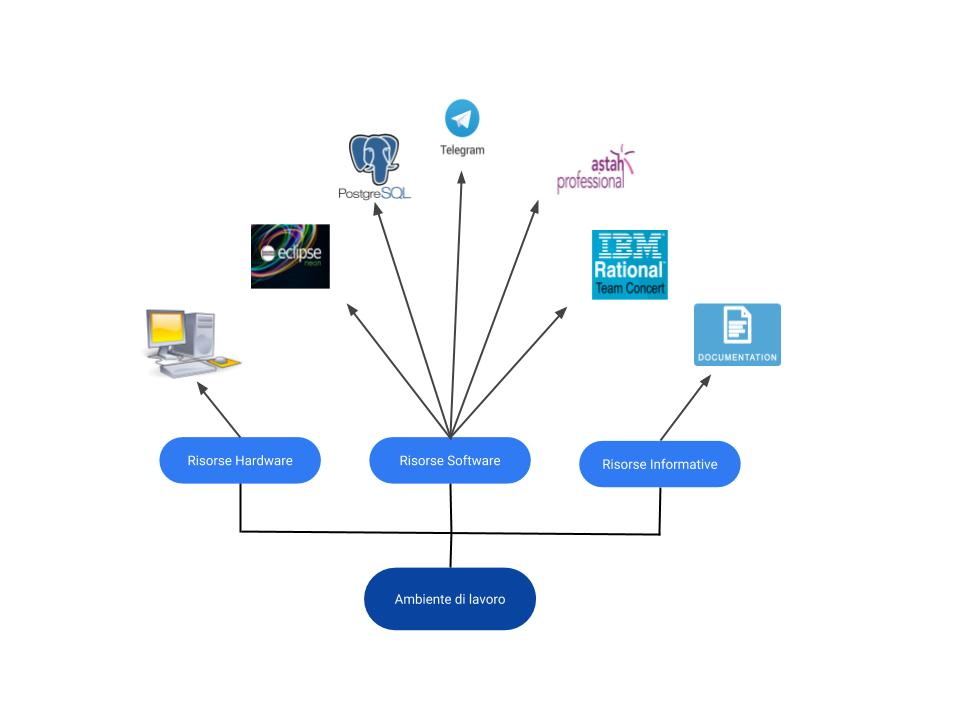
\includegraphics[scale=0.43]{ambiente_di_lavoro} 
    \caption{Ambiente di lavoro}
    \end{center}
 All'inizio dell'attività di stage, dall'azienda Sanmarco Informatica S.p.A. ho avuto accesso a diverse risorse dell'azienda per permettermi di eseguire il lavoro al meglio. \\
Le risorse condivise dall'azienda si suddividono in risorse hardware e risorse software, con i programmi messi a disposizione dall'azienda, e risorse informative, che comprendono i materiali di studio forniti inizialmente dall'azienda. 
\end{figure}  



\subsection{Risorse hardware}

Il team NextBI che fa parte nell'ambiente di Ricerca e Sviluppo dell'azienda Sanmarco Informatica S.p.A. mi ha seguito durante lo stage rendendomi il lavoro più facile con la loro collaborazione e disponibilità di formazione. \\

Mi è stato consegnato un PC aziendale già configurato con gli ambienti di lavoro aggiornati e alcuni software preinstallati per facilitare la fase di configurazione dell'ambiente. \\
Oltre al PC aziendale, mi è stato consentito l'utilizzo di una macchina virtuale per effettuare dei test necessari, molto utile soprattutto per l'esecuzione di ETL che richiedono tempi di esecuzione molto lunghi. 
\subsection{Risorse software}
Ho avuto accesso al repository aziendale basato su RTC il quale gestisce il versionamento del codice. I'RTC è stato configurato con l'IDE di Eclipse per garantire la compatibilità del sistema di versionamento già present nell'applicativo preesistente. \\
Il PC aziendale inoltre, aveva preinstallato la maggior parte dei software utili per effettuare il lavoro con versioni aggiornati. \\\\
Inoltre mi è stato consentito installare anche nuovi software, tools o librerie se necessari, a volte utili in particolari circostanze.

\subsection{Risorse informative}
Mi sono state fornite diverse risorse informative tra cui diverse note, manuali di programmazione  e la relativa documentazione dell'applicativo preesistente nel quale si va ad integrare il progetto di stage. Quest'ultimo ha favorito l'apprendimento corretto del funzionamento dell'applicativo preesistente a fine di ammortizzare i tempi di progettazione. 

\section{Tecnologie usate}
Sono varie le tecnologie usate durante lo stage. In questo paragrafo vengono descritte le diverse tecnologie usate con una breve presentazione. \\\\

\begin{enumerate}

\item \textbf{Java: }Java è un linguaggio di programmazione ad alto livello, orientato agli oggetti e a tipizzazione statica, specificatamente progettato per essere il più possibile indipendente dalla piattaforma di esecuzione.\\
La sua semplicità unita all'essere un linguaggio multi piattaforma lo rende molto usato e fa si che disponga di un'elevata quantità di librerie facilmente integrabili per le attività varie.\\
Uno dei principi fondamentali del linguaggio Java è espresso dal motto WORA (write once, run anywhere, ossia "scrivi una volta, esegui ovunque"): il codice compilato che viene eseguito su una piattaforma non deve essere ricompilato per essere eseguito su una piattaforma diversa. Il prodotto della compilazione è infatti in un formato chiamato bytecode che può essere eseguito da una qualunque implementazione di un processore virtuale detto Java Virtual Machine. 
Al 2014, Java risulta essere uno dei linguaggi di programmazione più usati al mondo, specialmente per applicazioni client-server, con un  numero di sviluppatori stimato intorno ai 9 milioni.\\\\

\item \textbf{XML (Extensible Markup Language) : }XML è un linguaggio di markup che definisce regole per la codifica di documenti in un formato comprensibile sia se letto da un umano che da una macchina. Lo scopo principale del formato è concentrato sulla semplicità, generalità e usabilità generale. Il formato permette quindi di definire tag personalizzati per i vari campi e mantenere un output che sia analizzabile in maniera automatica e manuale.
Il formato è stato usato perchè già integrato all'interno del Plug-in MyBatis per generare gli oggetti DAO corrispondenti alle tabelle del database.

\item \textbf{PostgresSQL :}
PostgreSQL è un completo modello di base di dati (\gls{DBMS}) ad oggetti rilasciato con licenza libera (stile Licenza BSD).\\
PostgreSQL è una reale alternativa sia rispetto ad altri prodotti liberi come MySQL, Firebird SQL che a quelli a codice chiuso come Oracle, IBM o DB2 ed offre caratteristiche uniche nel suo genere che lo pongono per alcuni aspetti all'avanguardia nel settore dei database.\\
PostgresSQL è stato utile nel progetto poichè ha permesso di collegare diversi database e farli comunicare tra loro con un'interfaccia facile da manovrare.\\
PostgreSQL, inoltre, permette l'ereditarietà dei tipi, uno dei principali concetti della programmazione orientata agli oggetti\\
Infine, con PostgreSQL si può implementare la logica in uno dei molti linguaggi supportati.

\item \textbf{Notepad++ : } Notepad++ è un text editor \gls{open source} mirato alla modifica di codice sorgente. Il programma non dispone di tutte le capacità di un vero IDE ma presenta funzionalità più basilari come syntax highlighting (evidenziazione della sintassi) per 
vari linguaggi tra cui anche Java, ricerca avanzata anche tramite espressioni regolari e la possibilità di aggiungere diversi plugin per espanderne le capacità.
Notepad++ si è rivelato molto utile sia come semplice text editor ma anche per permettere rapide modifiche al codice grazie alla maggiore rapidità presentata rispetto a Eclisse.

\item \textbf{Astah Community Astah Community: } Astah è un programma per la modellazione di schemi UML (Unified Modeling Language) cioè rispettanti degli standard industriali per i modelli general-purpose per l'ingegneria del software.
Il programma è stato scelto perchè ritenuto abbastanza semplice da usare per lo scopo necessario dopo esperienze precedenti ed è stato usato per creare alcuni diagrammi durante la fase di progettazione.

\item \textbf{Evernote :} Evernote è un programma multi piattaforma mirato alla creazione di note, la loro organizzazione, archiviazione e condivisione. Dispone sia di client installabile sia di un'interfaccia web e permette anche di condividere piccoli file.
L'uso del programma è stato richiesto da parte del tutor ed è servito per parte del processo di documentazione. Su di esso sono stati infatti tenute cronologie, appunti e tracce delle decisioni che sono state fatte man mano durante il proseguimento dello stage.

\item \textbf{Visual Studio Code :}
Visual Studio Code è un editor di codice sorgente sviluppato da Microsoft compatibile cin diversi sistemi operativi.
Visual Studio Code è basato su Electron, un \gls{framework} con cui è possibile sviluppare applicazioni Node.js.\\
Questo editor supporta vari linguaggi di programmazione, tra cui anche JavaScript e Java.
Visual Studio Code permette installare varie estensioni, con la possibilità di fare ciò direttamente dal programma. \\
Il software Visual Studio è stato usato principalmente per facilitare lo sviluppo front-end grazie alle sue numerose estensioni disponibili facilmente instancabili. 

\item \textbf{Telegram :} Telegram è un servizio di messaggistica istantanea basato su cloud ed erogato senza fini di lucro dalla società Telegram LLC. I client ufficiali di Telegram sono distribuiti come software libero per diverse piattaforme. \\\\
Da giugno 2015 Telegram ha introdotto una piattaforma per permettere, a sviluppatori terzi, di creare i Bot. I Bot sono degli account Telegram, gestiti da un programma, che offrono molteplici funzionalità con risposte immediate e completamente automatizzate. Grazie a questa funzionalità, il Bot telegrma è diventata la piattaforma dove si basa la maggior parte dell'applicativo sviluppato durante il periodo dello stage.

\item \textbf{FileZilla :} FileZilla Client è un software libero multipiattaforma che permette il trasferimento di file in Rete attraverso il protocollo FTP. Il programma è disponibile per GNU/Linux, Microsoft Windows, e macOS. Tra i vari protocolli supportati, oltre all'FTP vi è l'SFTP, e l'FTP su SSL/TLS. 
Il codice sorgente di FileZilla è disponibile sul sito SourceForge e, in alcuni casi, anche al momento dell'installazione del programma. Il progetto fu nominato Progetto del Mese nel novembre del 2003.\\
Questo software è stato usato nel periodo dello stage per poter permettere dei trasferimenti di diversi file dal server dell'azienda Sanmarco Informatica a quello dei clienti dove è stato installata la demo. \\


\end{enumerate} 






















             % Processi
% !TEX encoding = UTF-8
% !TEX TS-program = pdflatex
% !TEX root = ../tesi.tex

%**************************************************************
\chapter{Definizione del problema}
\label{cap:definizione-problema}
%**************************************************************

\intro{Breve introduzione al capitolo}\\

%**************************************************************


%**************************************************************
\section{Sempre più portabilità}


Quando le attività da gestire in un'azienda diventano tante, si ha la necessità di tenerle sotto controllo molte volte durante la giornata e questo purtroppo richiede quasi sempre un PC o tablet per poterci accedere attraverso una pagina web. Questo problema lo ritroviamo in tanti altri sistemi dove si richiede l'utilizzo di un'interfaccia web per interagire. Eliminando l'interfaccia web sostituendola con un applicazione installabile a volte non è la soluzione migliore perché questo significa dover fornire una funzionalità a tutte le piattaforme e sistemi operativi disponibili altrimenti si  limiterebbe il supporto delle funzionalità solo su una specifica piattaforma o sistema operativo. Bisognerebbe quindi trovare un modo per rendere l'applicativo un'applicazione portabile, cioè senza il bisogno dell'installazione e questo problema viene affrontato nel prossimo capito.

\section{Il problema della notificazione}

Nell'applicativo preesistente non è presente  la possibilità di notificare l'utente in tempo reale quando succede qualcosa su un certo evento programmato.  Questa estensione sarebbe molto apprezzata nel nuovo applicativo. Fornire un sistema di notificazione significa creare degli eventi e restare in ascolto su di essi finché non succeda qualcosa per scaturire l'evento. \\

Negli ultimi tempi di internet, queste funzionalità hanno preso piede in diversi ambiti. Oggigiorno grazie alle “Notification API” siamo in grado di inviare delle notifiche sfruttando il sistema operativo che sta usando il nostro utente. Possiamo creare ad esempio una chat online, come Slack, e sfruttare le notifiche per avvertire l'utente che ha ricevuto un nuovo task da portare al termine, oppure possiamo creare all'interno della nostra applicazione web un ToDo List, come “Asana”, per ricordare all'utente che si sta avvicinando la scadenza di un determinato task.\\
Questo tipo di notifiche sono molto interessanti per diverse tipologie di applicazioni web ma il primo problema da affrontare con le applicazioni web è la compatibilità delle “Notifications API”  con i vecchi  browser essendo questa tecnologia relativamente recente. Anche questo problema sarà affrontato nel prossimo capitolo.


\section{L'aggiornamento in real time}
Le aziende che si occupano di gestionale si trovano quasi sempre a gestire dati molto importanti e sensibili di altre aziende. Per questo motivo il software gestionale limita l'accesso e modifica dei dati nel database secondo la propria politica di gestione. Per poter interfacciarsi con questo problema bisogna trovare un sistema che faccia una specie di "backup" delle tabelle di interesse del gestionale sul quale effettuarci le query e successivamente portarle nel database gestionale di origine. A questo punto si presenta due problemi fondamentali: il primo problema è quello della gestione della mutua esclusione del dato, ovvero cosa succede se due utenti modificano lo stesso campo nello stesso istante di tempo? Come rispecchiare queste modifiche nel database di origine? Il secondo problema è quello di capire ogni quanto tempo bisogna fare l'aggiornamento delle tabelle dal database gestione. Quest'ultimo problema influisce direttamente sulle performance dell'applicativo poichè, come specificato sopra, i dati devono essere aggiornati il più possibile nel momento in cui si effettua una richiesta dall'interfaccia utente. Ma dall'altra parte, aggiornando le tabelle ogni secondo richiederebbe tanta velocità di calcolo. Bisogna dunque trovare un compromesso ragionevole. 

\section{Trasformazione dei dati}
Un altro problema da affrontare è quello di effettuare delle trasformazioni dei dati in altri formati. Spesso nei sistemi gestionali è richiesta una rappresentazione dei dati dal database in diversi formati come ad esempio in XML, Doc, PDF eccetera.  \\
Come descritto nel prossimo capito questo problema vine affrontato con il sistema ETL, più specificamente verrà usato il software di PDI (Pentaho Data Integration) chiamto Kettle.






\section{Analisi del problema e soluzione}


\subsection{Studio iniziale del problema di portabilità}
Dopo una attenta analisi per quanto riguarda il problema della portabilità dell'applicativo, è stato deciso sin dal primo tentativo di affiancare l'interfacci web esistente con una mobile. Questa decisione si basa sul fatto che avere un'interfaccia mobile è sempre comodo da usare e portare con se, dato che al giorno d'oggi, tutti possediamo uno smartphone personale sempre con noi. E' stata esclusa subito invece la possibilità di creare un'applicazione mobile da zero. Questo perchè come descritto nel primo capitolo si cerca di avere una soluzione capace di fornire un'applicativo dinamico, di facile utilizzo, che includa un sistema di notificazione per gli eventi preimpostati, che non abbia bisogno di essere installato e sopratutto che non abbia nessun tipo di dipendenza dal sistema operativo o browser.\\ 
 In secondo luogo è stata analizzata la possibilità di utilizzare una piattaforma già pronta open source che implementi un modulo di messaggistica chat, capace di ospitare il nostro sistema di notificazione attraverso l'invio di messaggi, evitando cosi di realizzare uno tutto da zero.\\\\
Navigando su internet si trovano decine di chat application open source che possono andar bene al caso nosto. Tra le più utilizzate sono: \\\\

\begin{itemize}
\item Slack 
\item RocketChat
\item IRC
\item Let's Chat
\item Telegram 
\item ecc...
\end{itemize}


\subsubsection{Scelta della Chat Application}
Valutando le funzionalità offerte dalla lista delle Chat Application è stato scelto Telegram come servizio di messaggistica di appoggio. Recentemente Telegram ha introdotto una nuova piattaforma per permettere agli sviluppatori di creare i Bot. I Bot sono degli account Telegram, gestiti da un programma, che offrono molteplici funzionalità con risposte immediate e completamente automatizzate. \\\\
Uno dei motivi principali per cui è stata presa questa decisione è la guida completa e la dettagliata documentazione del codice sorgente fornita dai membri Telegram. Grazie ai numerosi sviluppatori e membri attivi telegram, è sempre più facile trovare una risposta ai problemi nei appositi forum oppure contattando direttamente i loro membri.\\ Telegram supporta lo sviluppo con la maggior parte dei linguaggi di programmazione tradizionali (non solo OOP), tra i quali Java. Questo ha reso ancora più facile la nostra scelta nel progetto. \\

qui verrano aggiunti altri dettagli della scelta telegram .....


\subsection{Il problema dell'aggiornamento dei dati in real time}

Per ovviare questo problema è stato deciso di realizzare degli script i quali fanno partire dei processi per aggiornare le tabelle di interesse sistematicamente in un orario prefisato. L'applicazione Kettle fornito dall'impresa Pentaho, è stato un tool programmabile molto utile nel gestire i processi di lettura ed aggiornamento delle tabelle. In queto modo i dati saranno aggiornati nel database dell'applicativo e poichè le operazione effettuate dall'utente sono prevalentemente di lettura (dall'interfaccia web invece non è cosi), il problema della mutua esclusione  non si presenta in questo scenario. 

\subsection{L'associazione B2B - Telegram}
Come vedremo nella progettazione le operazioni che andranno a scrivere sul database sono quelle che si occupano di creare un'associazione tra l'utente B2B e quello dell'account Telegram. Il database sul quale verrano memorizzati gli account degli utenti è diverso da quello che conterrà i dati del B2B. Questa separazione servirà per garantire un'identificazione univoca degli utenti B2B con quelli registrati con il Bot Telegram. Inoltre verrà utilizzato lo stesso database che si occupa della gestione degli utenti, per gestire anche le licenze e la loro validità per ciascun utente. In questo caso l'unico utente che modificherà e attiverà le license sarà l'utente amministratore per cui siamo sicuri che non si presenterà nessun problema di sincronizzazione e modifiche multiple da parte di più utenti. 

\subsection{La  soluzione scelta per la trasformazione dei dati}

Per quanto riguarda le trasformazioni ETL dei dati è stato scelto di utilizzare il software Kettle il quale è un software molto affidabile e presenta un'interfaccia molto intuitiva. Grazie a Kettle è stato possibile estrarre i dati dalla sorgentie gestionale ed elaborarli ulteriormente facendoli subire le trasformazioni desiderate. Le più comuni trasformazioni sono state: la normalizzazione dei dati, l'eliminazione dei duplicati, la derivazione dei nuovi calcolati, il raggruppamento degli stessi selezionando quelli di interesse eccetera. \\

........































             % Kick-Off
% !TEX encoding = UTF-8
% !TEX TS-program = pdflatex
% !TEX root = ../tesi.tex

%**************************************************************
\chapter{Analisi dei requisiti}
\label{cap:analisi-requisiti}
%**************************************************************

\intro{Il quarto capitolo descrive in maggiore dettaglio il lavoro eseguito durante lo stage, le varie soluzioni che sono state considerate e come queste sono state scelte e composte per progettare la soluzione ideale.}\\






\section{Casi d'uso}

In questa sezione vengono trattati i casi d'uso riguardanti l'interazione dell'utente con l'interfaccia visiva dell'applicativo. Con i casi d'uso si vuole mostrare una panoramica delle funzionalità dell'applicativo. Vengono inseriti gli Use Cases Diagram e la loro descrizione secondo le specifiche UML2.0. L'attore principale è sempre l'utente generico autenticato oppure l'utente  amministrativo autenticato.
\begin{figure}[h!]
\subsection{Pagina iniziale } 
   \begin{center}
    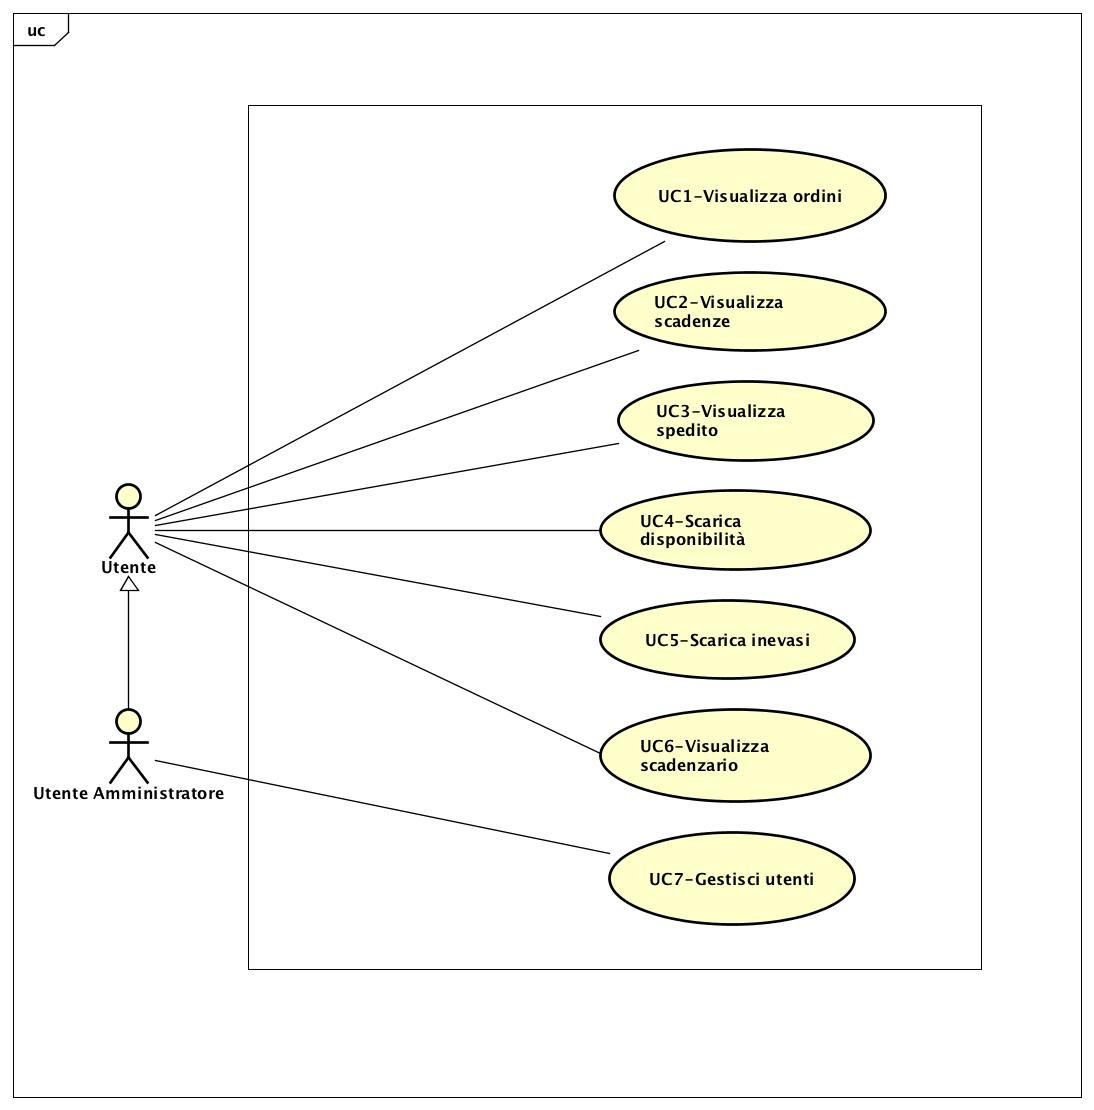
\includegraphics[scale=0.28]{usecase/UseCase_Diagram0} 
    \caption{Use Case - UC0: Scenario principale}
    \end{center}



\textbf{Attori primari:}   Utente autenticato\\

\textbf{Descrizione:} L'utente generico può visualizzare la lista degli ordini, può visualizzare le scadenze, lo spedito, la disponibilità degli ordini, gli inevasi e lo scadenzario. L'utente amministratore (che è una generalizzazione dell'utente generico) può gestire gli utenti, attivando una licenza, rimuovere gli utenti, associare un utente con un account B2B e rimuovere un'associazione. \\

\textbf{Precondizione:}  Il sistema funziona correttamente e visualizza la pagina principale correttamente. \\

\textbf{Postcondizione:} Il sistema ha ricevuto uno dei comandi eseguiti dall'utente ed è stato scaricato il file che visualizza le informazioni richieste dall'utente oppure è stato aperta la pagina dell'amministrazione degli utenti nel caso dell'utente amministratore.\\


\textbf{Flusso base degli eventi:}   
\begin{itemize}
\item L'attore visualizza la lista del tipo di ordine da selezionare (UC1);
\item L'attore può visualizzare la lista del tipo di scadenze da selezionare (UC2);
\item L'attore può visualizzare la lista del tipo di spedito da selezionare (UC3);
\item L'attore può scaricare il documento aggiornato  del report di Disponibilità (UC4);
\item L'attore può scaricare il documento aggiornato del report Inevaso (UC5);
\item L'attore può visualizzare la lista del tipo di scadenzario da selezionare (UC6);
\item L'attore (utente amministratore) può visualizzare la lista dei comandi per gestire l'associazione tra utenti, l'eliminazione e la gestione delle licenze (UC7);
\end{itemize}
\end{figure}




\begin{figure}[h!]
\subsection{Amministrazioni utenti}
   \begin{center}
    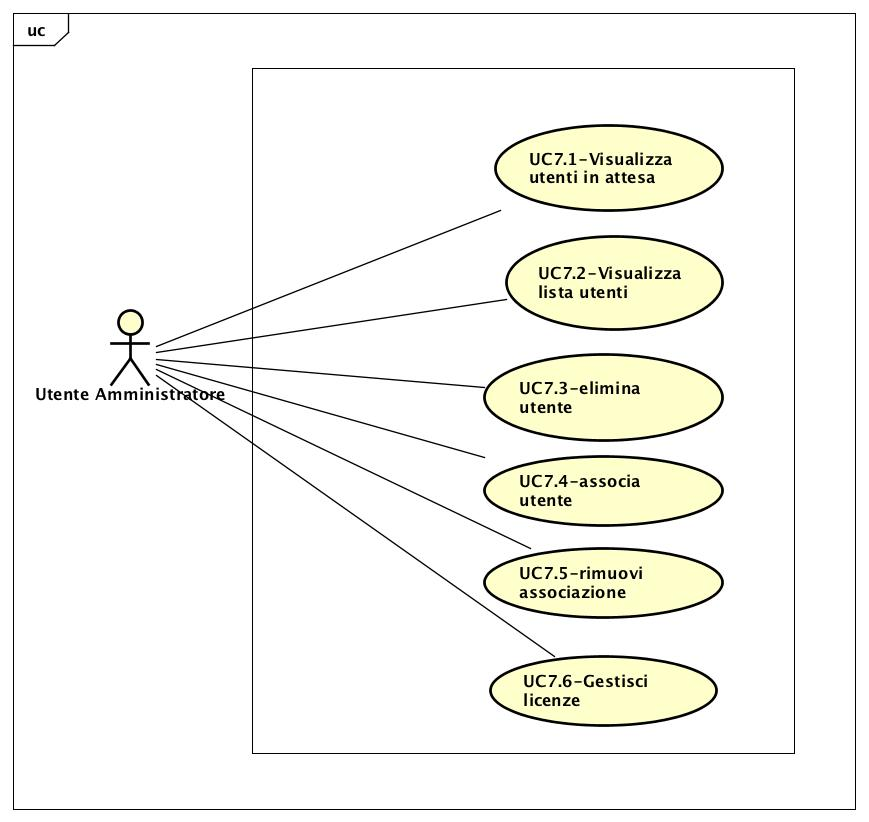
\includegraphics[scale=0.32]{usecase/UseCase_Diagram1} 
    \caption{Use Case - UC7: Area amministrativa}
    \end{center}
    
    \textbf{Attori primari:}   Utente amministratore autenticato\\
    
\textbf{Descrizione:} L'utente amministratore può visualizzare la lista degli utenti che risultano attivi con una licenza, visualizzare gli utenti che sono in attesa ad essere registrati nel sistema (cioè gli utenti che hanno fatto richiesta per essere registrati con una licenza ma che non sono ancora accettati da un amministratore). L'utente amministratore può eliminare un utente generico può gestire la licenza, inserendo una nuova oppure visualizzare lo stato di quelle attive. Infine l'utente amministratore può effettuare un'associazione tra l'utente B2B ed il suo account telegram oppure può eliminare un'associazione precedentemente creata. \\

\textbf{Precondizione:}   Il sistema funziona correttamente e visualizza la pagina all'amministrazione utenti correttamente. \\

\textbf{Postcondizione:}  L'utente amministratore è stato in grado ad effettuare correttamente  un'operazione da lui voluta nella pagina di gestione utenti.\\


\textbf{Flusso base degli eventi:} 

\begin{itemize}

\item L'utente amministratore visualizza la lista degli utenti in attesa ad essere registrati (UC7.1);
\item L'utente amministrativo visualizza la lista degli utenti registrati correttamente con una licenza valida (UC7.2);
\item L'utente amministrativo elimina un utente rimuovendo anche la relativa licenza (UC7.3);
\item L'utente amministrativo associa un utente B2B con il suo account telegram (UC7.4);
\item L'utente amministrativo rimuove l'associazione di un utente B2B con l'account telegram (UC7.5);
\item L'utente visualizza la lista dei comandi per l'amministrazione di un utente generico (UC7.6);
\end{itemize}  

\end{figure}






\begin{figure}[h!]
\subsection{Ordini del giorni}

   \begin{center}
    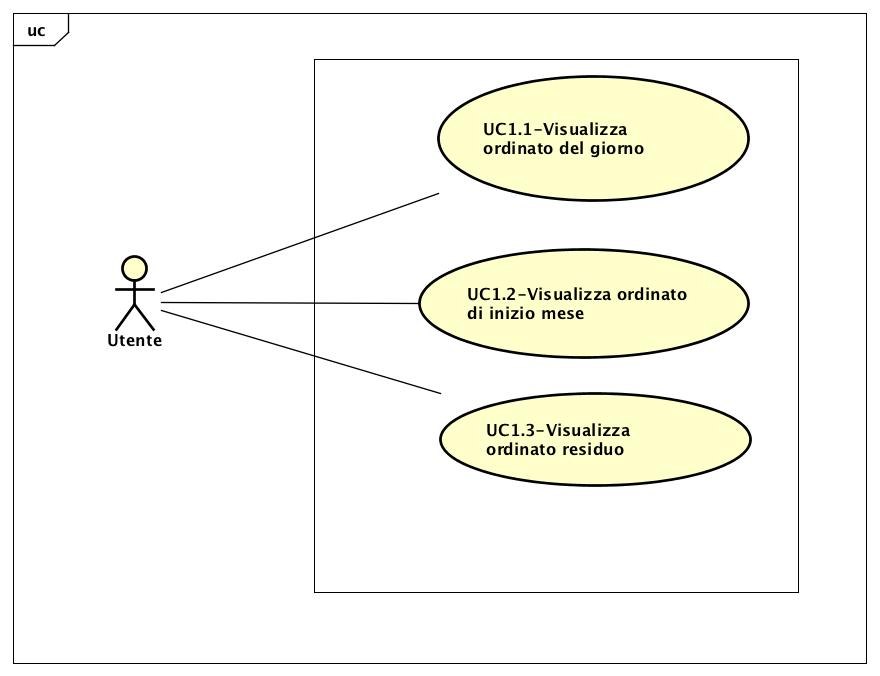
\includegraphics[scale=0.35]{usecase/UseCase_Diagram2} 
    \caption{Use Case - UC1: Ordini del giorno}
    \end{center}



\textbf{Attori primari:} Utente generico ed utente amministratore autenticati
\\


\textbf{Descrizione:} L'utente (generico oppure amministratore) può scegliere di visualizzare il report "ordinato del giorno", "ordinato di inizio mese" o "ordinato residuo". \\

\textbf{Precondizione:} Il sistema funziona correttamente e visualizza la pagina per poter scaricare gli ordinati correttamente. \\

\textbf{Postcondizione:}  L'utente generico oppure amministratore è stato in grado di visualizzare correttamente  un "ordinato" da lui voluto nella pagina di visualizzazione ordini. \\


\textbf{Flusso base degli eventi:} 

\begin{itemize}
\item L'utente visualizza i valori inerente all'ordinato del giorno (UC1.1);
\item L'utente visualizza i valori inerente all'ordinato di inizio mese (UC1.2);
\item L'utente visualizza i valori inerente all'ordinato residuo (UC1.3);
\end{itemize}
\end{figure} 






\begin{figure}[h!]
\subsection{Scadenze}
   \begin{center}
    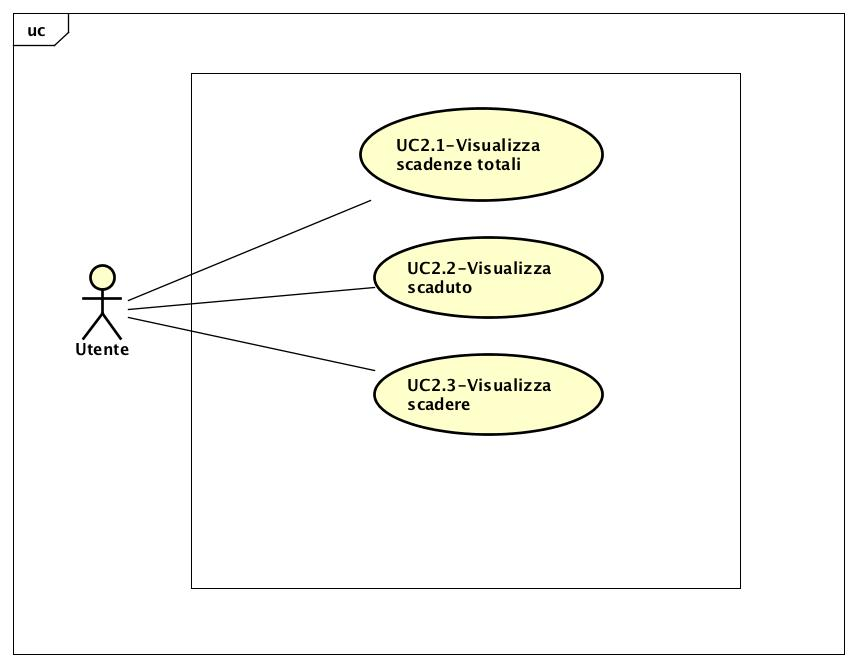
\includegraphics[scale=0.35]{usecase/UseCase_Diagram3} 
    \caption{Use Case - UC2: Scadenze}
    \end{center}

\textbf{Attori primari:} Utente generico ed utente amministratore autenticati
\\
\textbf{Descrizione:}  L'utente (generico oppure amministratore) può scegliere di visualizzare l'ammontare delle "scadenze totali", dello "scaduto" oppure "scadere".  \\

\textbf{Precondizione:} Il sistema funziona correttamente e visualizza la pagina per poter visualizzare le scadenze correttamente. \\

\textbf{Postcondizione:} L'utente generico oppure amministratore è stato in grado di visualizzare correttamente le scadenze da lui volute nella pagina di visualizzazione scadenze. \\


\textbf{Flusso base degli eventi:} 

\begin{itemize}
\item L'utente visualizza i valori inerenti alle scadenze totali (UC2.1);
\item L'utente visualizza i valori inerenti allo scaduto (UC2.2);
\item L'utente visualizza i valori inerenti allo scadere (UC2.3);
\end{itemize}
\end{figure}


\begin{figure}[h!]
\subsection{Gli spediti}
   \begin{center}
    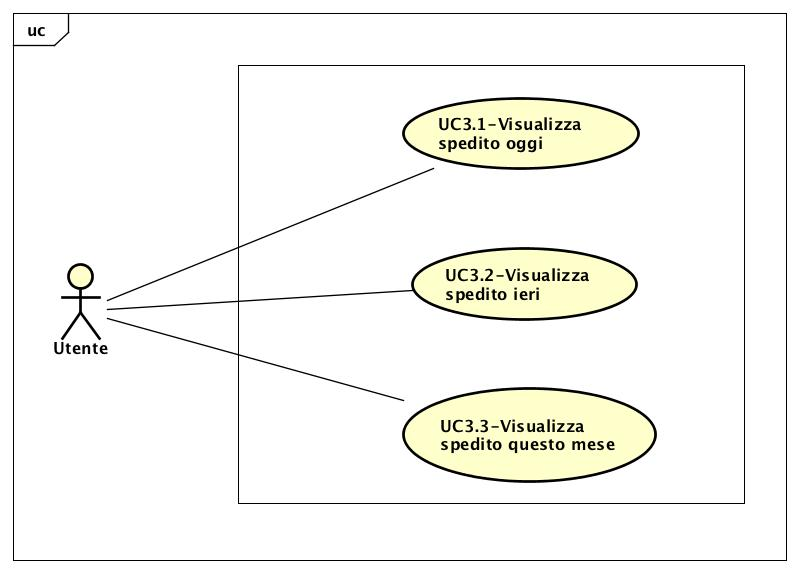
\includegraphics[scale=0.4]{usecase/UseCase_Diagram4} 
    \caption{Use Case - UC3: Scenario dello spedito}
    \end{center}


\textbf{Attori primari:} Utente generico ed utente amministratore autenticati
\\
\textbf{Descrizione:}  L'utente (generico oppure amministratore) può scegliere di visualizzare l'ammontare dello "spedito oggi", dello "spedito ieri" oppure "spedito questo mese".  \\

\textbf{Precondizione:} Il sistema funziona correttamente e visualizza la pagina per poter visualizzare gli spediti correttamente. \\

\textbf{Postcondizione:} L'utente generico oppure amministratore è stato in grado di visualizzare correttamente gli spediti da lui volute nella pagina di visualizzazione scadenze.  \\


\textbf{Flusso base degli eventi:} 

\begin{itemize}

\item L'utente visualizza i valori inerenti allo spedito oggi (UC3.1);
\item L'utente visualizza i valori inerenti allo spedito ieri (UC3.2);
\item L'utente visualizza i valori inerenti allo spedito questo mese (UC3.3);

\end{itemize}
\end{figure}



\begin{figure}[h!]
\subsection{Scadenzario}
   \begin{center}
    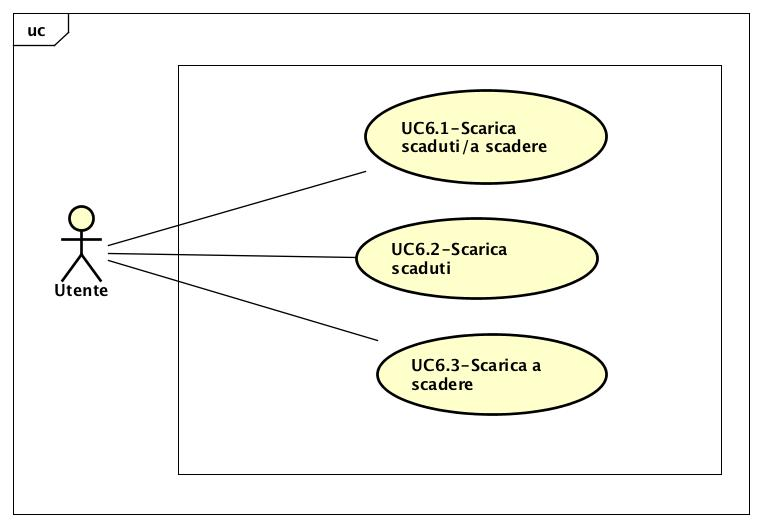
\includegraphics[scale=0.4]{usecase/UseCase_Diagram5} 
    \caption{Use Case - UC6: Scaduti/A scadere}
    \end{center}

\textbf{Attori primari:} Utente generico ed utente amministratore autenticati
\\


\textbf{Descrizione:}   L'utente (generico oppure amministratore) può scegliere di scaricare il documento che rappresenta il report di "scaduti/a scadere", "scaduti" oppure "a scadere".   \\

\textbf{Precondizione:}  Il sistema funziona correttamente e visualizza la pagina per poter scaricare lo scadenzario correttamente. \\

\textbf{Postcondizione:} L'utente generico oppure amministratore è stato in grado di scaricare correttamente lo scadenzario da lui volute nella pagina di visualizzazione scadenzario.  \\


\textbf{Flusso base degli eventi:} 

\begin{itemize}
\item L'utente scarica il report inerente agli scaduti/a scadere (UC6.1);
\item L'utente scarica il report inerente agli scaduti  (UC6.2);
\item L'utente scarica il report inerente allo scadere (UC6.3);
\end{itemize}
\end{figure}


\clearpage
\begin{table}
\begin{center}
\textbf{Tabella con requisiti funzionali}
\end{center}

\label{tab:requisiti-qualitativi}
\begin{tabular}{ |p{2cm}|p{8cm}|p{2cm}| }
 \hline
\textbf{ Requisito}   &  \textbf{Descrizione}    &  \textbf{    Use Case} \\ 
 \hline
  RF-0 &   L'attore può visualizzare la pagina principale per poter scegliere uno delle funzionalità presenti   & UC0 \\
 \hline
RF-1 &   L'attore visualizza la lista del tipo di ordine da selezionare (l'ammontare degli ordini in euro)  & UC1 \\
 \hline
 RF-2 & L'attore può visualizzare l'ordinato del giorno & UC1.1 \\
\hline
RF-3 & L'attore può visualizzare l'ordinato di inizio mese & UC1.2 \\
\hline
RF-4  &  L'attore può visualizzare l'ordinato residuo  & UC1.3 \\
\hline  
RF-5  & L'attore visualizza la lista del tipo di scadenze da selezionare  (l'ammontare delle scadenze in euro)  & UC2 \\
\hline
RF-6   & L'attore può visualizzare le scadenze totali   & UC2.1 \\
\hline
RF-7  &  L'attore può visualizzare lo scaduto & UC2.2 \\
\hline
RF-8   &  L'attore può visualizzare lo scadere & UC2.3 \\
\hline
RF-9   &  L'attore visualizza la lista del tipo di spedito da selezionare  (l'ammontare dello spedito in euro) & UC3 \\
 \hline
 RF-10   &  L'attore può visualizzare lo spedito di oggi & UC3.1 \\
  \hline
  RF-11   &  L'attore può visualizzare lo spedito di ieri & UC3.2 \\
   \hline
   RF-12  & L'attore può visualizzare lo spedito del mese  & UC3.3 \\
   \hline
   RF-13  &  L'attore può scaricare il documento aggiornato del report di Disponibilità & UC4 \\
   \hline
   RF-14  & L'attore può scaricare il documento aggiornato del report Inevaso   & UC6 \\
   \hline
RF-15    &  L'attore può visualizzare la lista dei comandi per gestire l'associazione tra utenti, l'eliminazione e la gestione delle licenze & UC7 \\
 \hline
   RF-16     & L'attore può visualizzare gli utenti in attesa di registrazione   & UC7.1 \\
\hline
RF-17   & L'attore può visualizzare la lista gli utenti già registrati   & UC7.2 \\
\hline
RF-18   & L'attore può eliminare un utente  & UC7.3 \\
\hline
RF-19   &  L'attore può associare un utente B2B con il suo account telegram  & UC7.4 \\
\hline
RF-20  &  L'attore può rimuovere l'associazione di un utente B2B con il suo account telegram & UC7.5 \\
\hline
RF-21   &  L'attore può gestire la licenza di un utente  & UC7.6 \\
\hline
RF-22   &  L'attore può visualizzare le licenze degli utenti & UC7.7 \\
\hline
RF-23   & L'attore può inserire una  licenza  & UC7.8 \\
\hline
\end{tabular}
\\
\caption{Tabella del tracciamento dei requisiti funzionali}
\end{table}



\begin{table}
\begin{center}
\textbf{Tabella con requisiti qualitativi}
\end{center}
\begin{tabular}{ |p{2cm}|p{8cm}|p{2cm}| }
 \hline
\textbf{ Requisito}   &  \textbf{Descrizione}    &  \textbf{    Use Case} \\ 
\hline
RQ-1  &  Il codice sviluppato deve essere versionato con il sistema RTC integrato nello strumento Eclipse & Azienda \\
\hline
RQ-2 &  Si deve usare il software Kettle per la gestione ETL & Azienda \\
\hline
\end{tabular}
\\
\caption{Tabella con requisiti qualitativi}
\end{table}




\begin{table}
\begin{center}
\textbf{Tabella dei vincoli}
\end{center}
\begin{tabular}{ |p{2cm}|p{8cm}|p{2cm}| }
 \hline
\textbf{ Requisito}   &  \textbf{Descrizione}    &  \textbf{    Use Case} \\ 
\hline

RV-1 &  Il prodotto deve essere sviluppato secondo rispettando  gli standard ISO aziendali & Azienda \\
\hline
RV-2 &  L'interfaccia front-end deve essere sviluppata, basandosi sulla piattaforma telegram per sfruttare le notifiche push  & Azienda \\
\hline
RV-3 &  La logica di BI deve essere sviluppata come web-services sul server Java Tomcat& Azienda \\
\hline
RV-4 & Come DBMS si deve usare PostgresSQL & Azienda \\
\hline
\end{tabular}
\\
\caption{Tabella dei vincoli}
\end{table}










             % Concept Preview
% !TEX encoding = UTF-8
% !TEX TS-program = pdflatex
% !TEX root = ../tesi.tex

%**************************************************************
\chapter{Progettazione e codifica}
\label{cap:progettazione-codifica}
%**************************************************************

\intro{
In questo capitolo vengono descritte le principali scelte progettuali, la struttura del database, la struttura del server e dell'applicativo client-side.}\\

%**************************************************************
%\section{Tecnologie e strumenti}
%\label{sec:tecnologie-strumenti}

%Di seguito viene data una panoramica delle tecnologie e strumenti utilizzati.

%\subsection*{Tecnologia 1}
%Descrizione Tecnologia 1.

%\subsection*{Tecnologia 2}
%Descrizione Tecnologia 2

%**************************************************************


\begin{figure}[h!]
\section{Database}
\label{sec:database}

Per gestire l'area di amministrazione degli utenti è stato costruito il database locale di amministrazione chiamato "data", appunto perché dovrà rappresenta tutti i dati amministrativi dell'utente, la gestione dell'associazione tra utenti b2b con quelli di telegram, le licenze degli utenti e tutta la gestione della tastiera telegram. La creazione e la  gestione della tastiera di telegram è automatizzata dalla tabella Keyboard, ovvero per creare un nuovo tasto associato ad una funzionalità, bisogna semplicemente scrivere sulla tabella Keyboard il nome del tasto, su quale riga si vuole posizionare e il nome del metodo che verrà chiamato quando si preme quel bottone. Questo sistema di gestione di tastiera è molto comodo per tenere una separazione tra i vari componenti che implementano una logica diversa. In questo modo è molto facile estendere l'applicativo con altre funzionalità modificando semplicemente una sola riga del database. 

   \begin{center}
     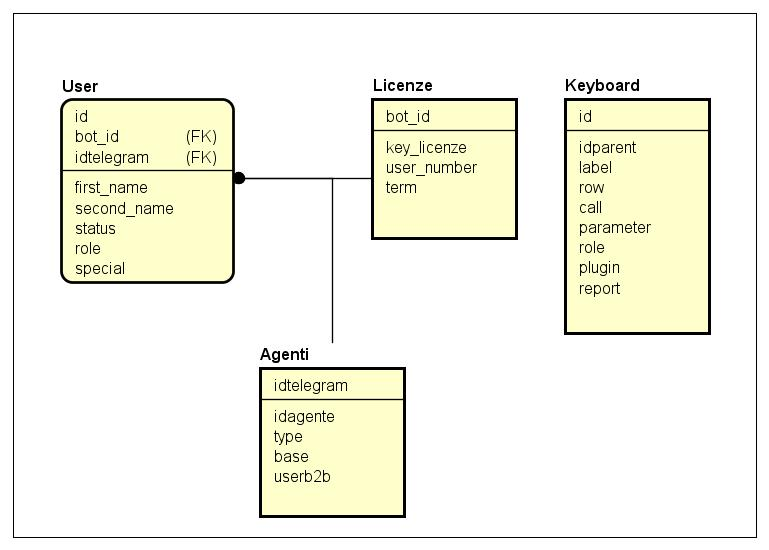
\includegraphics[scale=0.4]{diagrammi/database} 
    \caption{ER-Database }
    \end{center}

\subsection{Struttura}
In questa sottosezione verranno elencate tutte le tabelle che rappresentano la gestione dell'area amministrativa, spiegando il loro uso e funzionamento in modo da comprendere l'utilizzo che ne è stato fatto nel progetto per il salvataggio dei dati. \\
\end{figure}
\textbf{User} \\ 

In questa tabella vengono salvati i dati anagrafici dell'utente telegram,il suo ID identificativo univoco e il suo ruolo aziendale. \\

User ha i seguenti campi: \\ 
\begin{itemize}
\item \textbf{id:}  id univoco per identificare un univoco utente telegram;
\item \textbf{first\_name:} il nome dell'utente telegram;
\item \textbf{second\_name } il cognome dell'utente telegram;
\item \textbf{status:} lo status rappresenta se l'utente è abilitato "allow" oppure no, "deny";
\item \textbf{role:} role rappresenta il ruolo aziendale dell'utente;
\item \textbf{special:} special è un campo speciale utilizzato solo lato sviluppo per dare il massimo dei  permessi agli sviluppatore, utile in fase di testing;
\end{itemize}

\textbf{Agenti}\\

In questa tabella vengono salvati i dati riguardanti gli agenti, il loro Idtelegram, il loro tipo e la corrispondenza con il codice utente B2B.\\

La tabella Agenti presenta i seguenti campi:\\

\begin{itemize}
\item \textbf{id\_telegram:}  id univoco per identificare un univoco utente telegram;
\item \textbf{id\_agente:}  id univoco per identificare un agente;
\item \textbf{type:} rappresenta il tipo dell'agente;
\item \textbf{base:} rappresenta la base di appartenenza dell'agente;
\item \textbf{userb2b:} rappresenta il codice utente corrispondente in B2B;
\end{itemize}



\textbf{Licenze}
\\
In questa tabella vengono salvati i dati riguardanti le licenze con le loro scadenze per ciascun utente.\\

La tabella Licenze presenta i seguenti campi:

\begin{itemize}
\item \textbf{bot\_id:}  botid rappresenta l'ID univoco per identificare un utente telegram;
\item \textbf{key\_licenze:} rappresenta la chiave di licenza per gli utenti telegram;
\item \textbf{user\_number } rappresenta il numero massimo di account utilizzabili;
\item \textbf{term} rappresenta la data di scadenza della licenza;
\end{itemize}




\textbf{Keyboard}\\

In questa tabella vengono salvati i dati che riguardano la generazione della tastiera, la posizione e il nome del tasto.\\

La tabella Keyboard presenta i seguenti campi:\\

\begin{itemize}
\item \textbf{id:} id rappresenta l'ID associato al tasto univoco per identificare un utente telegram;
\item \textbf{id\_parent:} rappresenta la l'id del padre sul quale appendere il tasto;
\item \textbf{label } il campo label rappresenta l'etichetta del bottone;
\item \textbf{row } il campo row rappresenta il numero di riga dove si vuole aggiungere il tasto;
\item \textbf{call:} rappresenta la chiamata al metodo da effettuare quando si preme il bottone;
\item \textbf{parameter } parameter rappresenta i  parametri del metodo da chiamare
\item \textbf{role:} role rappresenta il ruolo dell'utente (admin oppure user);
\item \textbf{plugin } rappresenta il nome del plugin associato se c'è ne sono;
\item \textbf{report} rappresenta il nome del report;
\end{itemize}

\clearpage


\begin{figure}
\section{Back-end}
\label{sec:backend}
 \begin{center}
     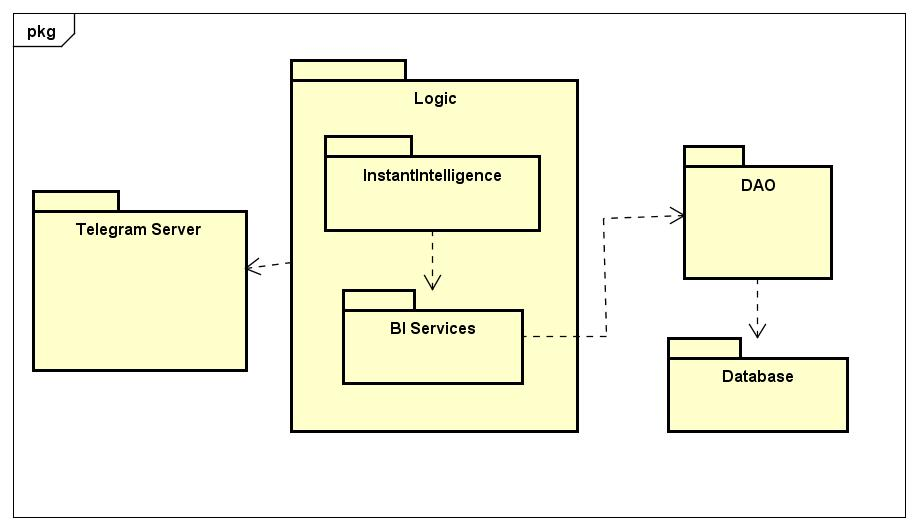
\includegraphics[scale=0.4]{diagrammi/Diagramm_backend} 
    \caption{Diagramma Back-end }
    \end{center}

\end{figure}  




\begin{figure}
\subsection{Server Telegram}
\label{sec:backend}
 \begin{center}
     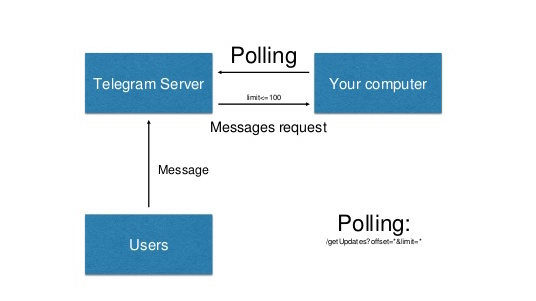
\includegraphics[scale=0.55]{diagrammi/polling} 
    \caption{Diagramm Polling }
    \end{center}

\end{figure}  






Nel progetto è stato implementato il metodo di long polling per le notifiche di telegram. Questo significa che ci si collega periodicamente al server telegram per aggiornarsi delle nuove notifiche. Come si vede nella prima figura, l'utente invia un messaggio ad un altro utente (in questo caso chiamato Your Computer). Il messaggio arriva al server telegram, il quale manda la richiesta al destinatario, dopodichè avviene il polling del messaggio verso il server. \\
Per la risposta invece il messaggio viene mandato prima al server telegram, successivamente viene mandato dal server all’utente desiderato.
\\Non possiamo dire nulla invece al riguardo del server telegram (il quale lo consideriamo come un Black-Box), poichè il codice sorgente del server telegram  non è disponibile ancora open source per il momento.


%


\subsection{InstantIntelligence}

Il package InstantIntelligence invece è la parte dove vengono elaborate le richieste dell'utente in base al tasto premuto. In questo package viene effettuato il controllo dell’autenticazione dell'utente, ovvero viene controllato se l’utente abbia una licenza valida oppure è la prima volta che sta accedendo e quindi sta chiedendo di essere abilitato.  Questo package si occupa anche della creazione e gestione della tastiera con i dati presi nel database Keyboard. Ogni richiesta fatta dall'utente, premendo un tasto oppure digitando un semplice comando passa per InstantIntelligence ed in base alla richiesta viene chiamato il relativo servizio BI, il quale si occuperà a sua volta di creare l'oggetto DAO corrispondente. \\\\

\subsubsection{Descrizione dei metodi più importanti}


\begin{itemize}
\item \textit{public void onUpdateReceived(Update update) :}  
questo metodo è il metodo che viene chiamato quando arriva un qualsiasi messaggio dall'utente telegram. Il parametro update invece è il contenuto del messaggio arrivato. I messaggi interessati nel nostro caso sono quelli che contengono una stringa come testo dato che il contenuto della stringa sarà fondamentale per chiamare successivamente il servizio giusto.

\item \textit{private boolean isWhiteListed(int id):}
il metodo isWhiteListed fà il controllo dell'utente se risulta registrato nella lista White dove sono memorizzati tutti gli utenti abilitati con una licenza. Il controllo viene effettuato sul parametro id dell'utente telegram. Se l'utente con codice id non fa parte della lisa White, viene mandato indietro un messaggio che avvisa l'utente di riprovare tra qualche minuto poichè si sta aspettando che un amministratore lo abiliti. 

\item \textit{private void handleIncomingMessage(Message message) :}
il metodo handleIncomingMessage è il gestore dei messaggi in arrivo e viene chiamato dopo il controllo del tipo di utente, ovvero se il metodo isWhiteListed ha ritornato true; 
handleIncomingMessage fà il paring sul contenuto del messaggio ed applica uno switch su  tutti i servizi da chiamare. Questo metodo ha il compito di costruire la tastiera iniziale se il "case" corrisponde al comando di "/start", altrimenti viene chiamato uno dei servizi, il quale prende la responsabilità di costruire la tastiera in base al comando ricevuto dal contenuto dell'oggetto Message.

	 \item \textit{private void onWelcomeMessage(String id, String firstName, ReplyKeyboardMarkup keyboardMarkup):} questo metodo contiene il messaggio iniziale di benvenuto e si occupa di caricare il menu principale da cui scegliere i vari processi. 

 \item \textit{private void onGetCommand(Message message, String queryResult):}
questo metodo gestisce tutti i comandi personalizzati e viene chiamato quando la query che si vuole fare risulta immediata e non necessita di un tasto nel menu.

 \item \textit{private void onGetReport(Message message, String call):}
onGetReport è il metodo che si occupa di inviare il report all’utente richiesto con la data e ora locale.

\item \textit{private static ReplyKeyboardMarkup getKeyboard(int idpadre):}
questo metodo si occupa di creare la tastiera corrente in base all'id padre rappresentato dalla tastiera appena nascosta quando è stato premuto un bottone. 

\item \textit{private static ReplyKeyboardMarkup getStartKeyboard():}
questo metodo costruisce la tastiera di start con i tasti predisposti in orizzontale.

\end{itemize}

\subsection{BI Services}

In questa sottosezione vengono descritti i servizi chiamati per creare e gestire i report. \\

\begin{itemize}

\item \textit{BDG\_Ordini\_Service:}Questo servizio si occupa di creare l'oggetto DAO che conterrà la lista degli ordini. Con un ciclo "for" si crea un unico oggetto di tipo stringa che rappresenta a secondo del DAO creato l'ordinato del giorno, l'ordinato di inizio mese oppure l'ordinato residuo. Il tipo di ritorno sarà una stringa poichè dovrà essere spedita al front-end come un messaggio di testo attraverso il metodo sendMessage(Message msg).

\item \textit{BDG\_Scadenze\_Service:}Questo servizio se occupa di creare e gestire le Scadenze che possono essere di tre tipi: Scadenze totali, Scaduto e Scadere. Anche questo servizio come BDG\_Ordini\_Service, in base alla richiesta dell'utente calcola e ritorna l'ammontare delle scadenze.

\item \textit{BDG\_Spedito\_Service:}BDG\_Spedito\_Service è uno dei tre servizi che si occupa di calcolare l'ammontare degli spediti che possono essere: Spedito oggi, Spedito ieri e Spedito questo mese. Questi tre servizi attualmente non fanno troppe operazione ma in futuro sono previsti calcoli più complessi.

\item \textit{BDG\_Disponibilità\_Service:}Questo servizio ha il compito di generare un documento con delle tabelle che contengono  la disponibilità degli articoli ordinati per codice articolo. BDG\_Disponibilità\_Service tiene conto della profilazione per codice agente.

\item \textit{BDG\_Inevasi\_Service:}Questo servizio genera il documento degli inevasi posizionando i dati in una tabella ordinati per numero di articolo. BDG\_Inevasi\_Service tiene conto della profilazione per codice agente.

\item \textit{BDG\_Scadenzario\_Service:}Questo servizio genera i documenti per lo scadenzario che possono essere di tre tipi: Scaduti, a scadere e insieme Scaduti/A scadere. BDG\_Scadenzario\_Service tiene conto della profilazione per codice agente.

\end{itemize}

\subsection{DAO}
Lo strato \gls{DAO} fondamentalmente ha una classe con relativi metodi che rappresenta
un'entità tabellare di un database e viene utilizzato per stratificare e isolare l'accesso
ad una tabella tramite query, che nel nostro caso sono costruite con una struttura Java
o interfacciandosi direttamente con il DAO. L'accesso al \gls{data-layer} da parte della
business-logic viene quindi controllato tramite DAO, creando un maggiore livello di
astrazione ed una più facile manutenibilità. I metodi del DAO con le rispettive query
verranno così richiamati dalle classi della business-logic.


\clearpage
\section{Front-end}

La parte Front-end di telegram è costituita principalmente dal menù principale che contiene i bottoni della tastiera, l'area di composizione del messaggio da inviare e l'area che visualizza la history della chat. In questa sezione si cerca di dare una panoramica generale di quelli che sono i componenti principali che compongono la tastiera interattiva dell'utente e i passi da seguire per poter portare a termine correttamente un operazione. Le figure saranno affiancate da una descrizione che illustra il funzionamento di vari componenti. 
Le operazioni che un utente può eseguire sono suddivisi in due blocchi: il primo contiene tutti i report disponibili e la loro gestione, il secondo blocco invece è accessibile solo dagli utenti amministratori e rappresenta la gestione dell'area amministrativa degli utenti generici. \\


\begin{figure}[h!]
\begin{center} \textbf{Menu principale} \end{center}
\begin{center}
    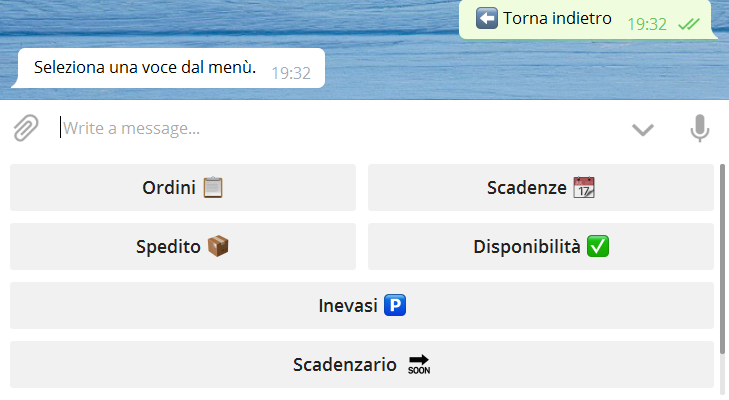
\includegraphics[scale=0.7]{screen/menu_principale} 
    \caption{Menu principale}
    \end{center}
Questa figura rappresenta il menu principale dove un utente generale può eseguire una delle operazioni disponibili nella tabella. Invece l'utente amministratore può accedere anche all'area amministrativa per la gestione delle licenze e l'associazione degli utenti. Per il bottone di Ordini, Scadenze e Spedizioni è presente l'ultimo livello dove l'utente può effettuare direttamente una richiesta di visualizzazione dell'ammontare (in euro) sul display. Per ciascun menù, all'ultima riga della tastiera è presente il tasto "Indietro"che permette di ritornare nel menù precedente. 
\end{figure}  




\begin{figure}[h!]
\begin{center}
\textbf{Menu Disponibilità}
\end{center}
\begin{center}
    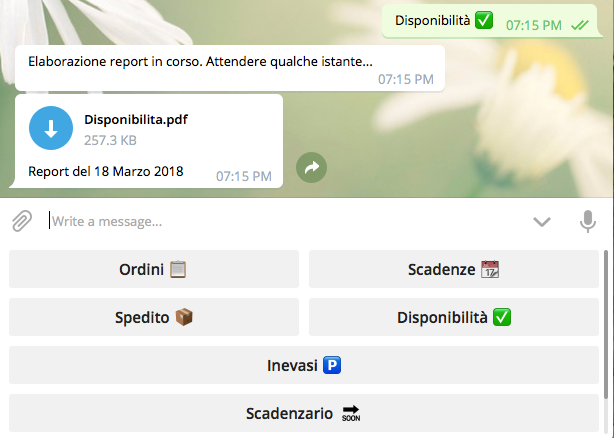
\includegraphics[scale=0.5]{screen/menu_disponibilita} 
    \caption{Menu Disponibilità}
     \end{center}
    Il bottone Disponibilità invece permette di scaricare direttamente il report di Disponibilità. Il report di disponibilità è profilato in base al tipo di utente, per cui la tabella che viene costruita in BI Service varia per utente. Lo stesso procedimento si ha anche per il bottone Inevasi. Lo scadenzario invece ha un altro livello innestato dove si può scegliere di scaricare il report totale di scadenze, quello scaduto oppure a scadere. Dal momento in cui il report viene scaricato è possibile visualizzarlo direttamente premendo un'altra volta sul nome del file senza evitando cosi di cercarlo nel file system del cellulare. Telegram gestisce diversi tipi di file di dimensione fino a 1.5GB e ciò permette di caricare anche file PDF di grandi dimensioni. 
\end{figure}  


\begin{figure}[h!]
   
    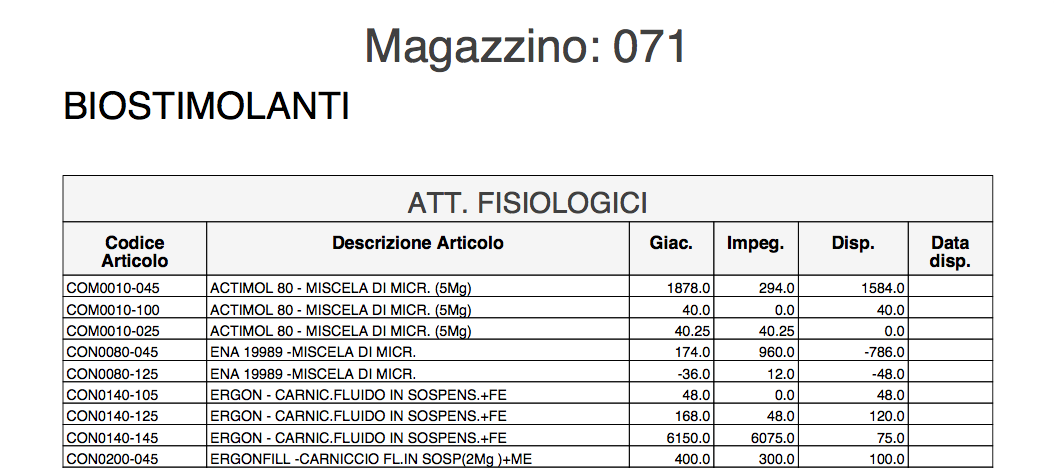
\includegraphics[scale=0.37]{screen/disponibilita} 
    \caption{Report Disponibilità}
     La figura 5.6 illustra una tabella che rappresenta la disponibilità giornaliera con il numero del magazzino e il codice identificativo dell’articolo in prima colonna.
\end{figure}  


\begin{figure}[h!]
   \begin{center}
   \textbf{Area amministrativa}\\
   \end{center}
   \begin{center}
    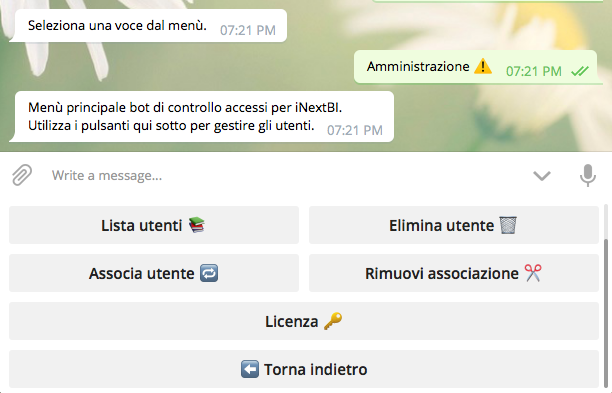
\includegraphics[scale=0.53]{screen/menu_admin} 
    \caption{Il menù di amministrazione}
    \end{center}
     Nella figura 5.7 vediamo invece come è composto il menù di amministrazione. In alto a sinistra troviamo la Lista utenti che visualizza sull'area della chat una lista degli utenti con i corrispondenti idTelegram che sono attualmente attivi e informazioni su eventuali associazioni con utenti B2B. In alto a destra invece il bottone Elimina utente permette di eliminare un utente non amministratore digitando semplicemente il suo idTelegram oppure il nome e cognome. 
\end{figure}  

\begin{figure}[h!]
   \begin{center}
   \textbf{Associazione utente B2B}\\
   \end{center}
   \begin{center}
    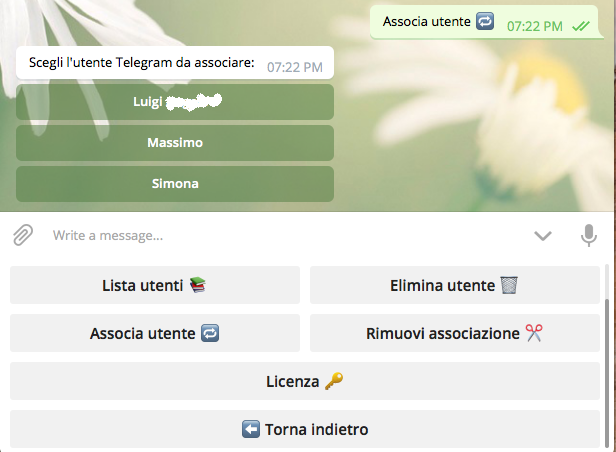
\includegraphics[scale=0.85]{screen/menu_associazione} 
    \caption{Associazione B2B}
    \end{center}
     Il menù di associazione utente permette di associare un id utente telegram con l'utente B2B facendo cosi in modo di avere un solo riferimento per utente. L'operazione di associazione avviene scegliendo prima un utente telegram da quelli che non risultano ancora associati. Per poter permettere all'utente amministratore di selezionare l'utente da associare è stata creata una tastiera inline con i nomi degli utenti. Premendo su un nome  si apre un'altra tastiera inline con le lettere dell'alfabeto. E’ sufficiente scegliere l'iniziale del nome dell'utente B2B per poterlo associare con quello di telegram.Per il bottone Rimuovi associazione invece abbiamo una sola lista di utenti associati rappresentati anche questi da un inline keyboard. Premendo su un nome, l'associazione utente telegram e utente B2B vine eliminata. 

\end{figure}  



\begin{figure}[h!]
   \begin{center}
   \textbf{Gestione Licenza}\\
   \end{center}
   \begin{center}
    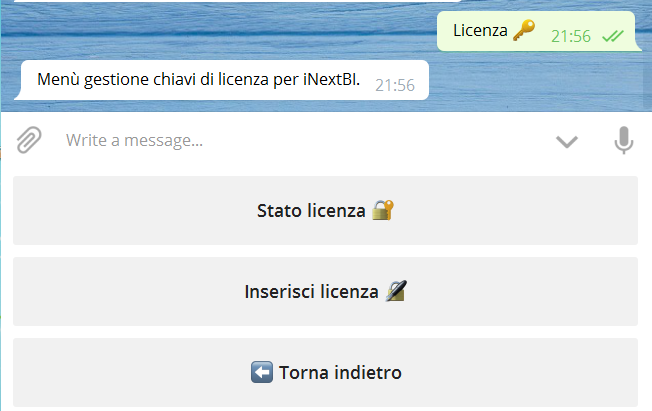
\includegraphics[scale=0.8]{screen/menu_licenza} 
    \caption{Licenze}
    \end{center}
   Per quanto riguarda il menù della licenza invece si hanno tre bottoni, il primo indica lo stato delle licenze per gli utenti generali, il secondo invece permette di inserire una licenza per gli utenti che si trovavano in stato di attesa. Dal momento che viene inserita una licenza valida, l'utente generico viene tolto dalla lista di attesa e può utilizzare le funzionalità dell'applicativo. Il terzo bottone invece permette di tornare al menù precedente.

\end{figure}  





             % Product Prototype
% !TEX encoding = UTF-8
% !TEX TS-program = pdflatex
% !TEX root = ../tesi.tex

%**************************************************************
\chapter{Conclusioni}
\label{cap:conclusioni}
%**************************************************************


%**************************************************************
\section{Raggiungimento degli obiettivi}
L'attività dello stage è terminata come previsto il 11/01/2018 senza particolari sforamenti. 
A fine stage è valutato il livello di raggiungimento degli obiettivi, dal quale tutti gli obiettivi obbligatori elencati nella tabella
 ???  risultano essere soddisfati. Gli obiettivi della tabella ??? nonostante pochi in numero, comprendono implicitamente a loro volta altri obiettivi il quale soddisfacimento ha richiesto quantità di tempo lavorativo non trascurabile. Per quanto riguarda gli obiettivi desiderabili, è stato soddisfato l'obiettivo con l'identificativo OB-9-D che consiste nel testare una serie di formule riassuntive dell'applicativo preesistente. E' rimasto invece non soddisfato l'obiettivo OB-10-D a causa dell'esaurimento delle ore prefissate nel documento piano di lavoro.

%**************************************************************
\section{Conoscenze acquisite}
Le conoscenze acquisiste durante il periodo di stage presso l'azienda Sanmarco Informatica S.p.A. sono state significative e di grande valore. Grazie all'utilizzo dei servizi offerti da telegram per la parte back-end, ho avuto la possibilità di acquisire conoscenze più approfondite per quanto riguarda il linguaggio di programmazione Java con il suo modello di programmazione orientata agli ogetti e uno studio più approfondito legato ai suoi algoritmi implemetati. Lavorando in un team composto da cinque persone sono stato in grado di comprendere quali sono le più comuni best practice da applicare su alcuni problemi riccorrenti e di capire  come ottenere una progettazione solida a partire da una buona raccolta dei requisiti funzionali; \\ Durante lo stage ho affrontato diversi argomenti che mi hanno portato allo studio di nuovi temi, come ad esempio lo studio del modello di Push Notification implementato nella piattaforma telegram, lo studio della libreria MyBatis che permette di interfacciarsi allo strato DBMS, l'acquisizione dei dati e scritture ETL attraverso il software Kettle e tanti altri. 

%**************************************************************
\section{Valutazione personale}

In conclusione l'attività dello stage è stata molto buona e soddisfacente. Nonostante le difficoltà iniziali incontrate nell’inserirsi all’interno di un progetto già esistente, il team di sviluppo NextBi mi ha affiancato e dato la possibilità di sentirmi a mio agio durante tutta l'attività. Ogni problema è stato affrontato con l'aiuto del tutor aziendale e il team di ricerca sempre disponibile.
L'attività dello stage mi ha permesso di cambiare il modo di affrontare alcuni problemi a livello di progettazione e mi ha insegnato come bisogna comportarsi difronte ad un problema reale e più ampio rispetto a quelli affrontati nel mondo accademico. Affermo che il prodotto finale è stato soddisfacente anche se su alcuni argomenti trattati sarebbe possibile ampliare il lavoro e probabilmente anche migliorarlo in alcuni aspetti.







              % Product Design Freeze e SOP
% !TEX encoding = UTF-8
% !TEX TS-program = pdflatex
% !TEX root = ../tesi.tex

%**************************************************************
\chapter{Conclusioni}
\label{cap:conclusioni}
%**************************************************************

%**************************************************************
\section{Consuntivo finale}

%**************************************************************
\section{Raggiungimento degli obiettivi}

%**************************************************************
\section{Conoscenze acquisite}

%**************************************************************
\section{Valutazione personale}
             % Conclusioni
\appendix                               
% !TEX encoding = UTF-8
% !TEX TS-program = pdflatex
% !TEX root = ../tesi.tex

%**************************************************************




             % Appendice A

%**************************************************************
% Materiale finale
%**************************************************************
\backmatter
\printglossaries
% !TEX encoding = UTF-8
% !TEX TS-program = pdflatex
% !TEX root = ../tesi.tex

%**************************************************************
% Bibliografia
%**************************************************************

\cleardoublepage
%\chapter{Bibliografia}

\nocite{*}
% Stampa i riferimenti bibliografici
\printbibliography[heading=subbibliography,title={Riferimenti bibliografici},type=book]

% Stampa i siti web consultati
\printbibliography[heading=subbibliography,title={Siti web consultati},type=online]


\end{document}